\begin{enumerate}[label=\thesection.\arabic*,ref=\thesection.\theenumi]
	\item A team of medical students doing their internship have to assist during surgeries
at a city hospital. The probabilities of surgeries rated as very-complex, complex,
routine, simple or very-simple are respectively, 0.15, 0.20, 0.31, 0.26, .08. Find
the probabilities that a particular surgery will be rated
\begin{enumerate}
\item complex or very-complex
\item neither very-complex nor very simple
\item routine or complex
\item routine or simple
\end{enumerate}
		\solution
		\iffalse
\def\inputGnumericTable{}
\let\negmedspace\undefined
\let\negthickspace\undefined
\documentclass[journal,12pt,twocolumn]{IEEEtran}
\usepackage{cite}
\usepackage{amsmath,amssymb,amsfonts,amsthm}
\usepackage{algorithmic}
\usepackage{graphicx}
\usepackage{textcomp}
\usepackage{xcolor}
\usepackage{txfonts}
\usepackage{listings}
\usepackage{enumitem}
\usepackage{mathtools}
\usepackage{gensymb}
\usepackage[breaklinks=true]{hyperref}
\usepackage{tkz-euclide} % loads  TikZ and tkz-base
\usepackage{listings}
\usepackage[latin1]{inputenc}
       \usepackage{fullpage}
       \usepackage{color}
       \usepackage{array}
       \usepackage{longtable}
       \usepackage{calc}
       \usepackage{multirow}
       \usepackage{hhline}
       \usepackage{ifthen}
       \usepackage{multirow}
\usepackage{adjustbox}



\DeclareMathOperator*{\Res}{Res}
\renewcommand\thesection{\arabic{section}}
\renewcommand\thesubsection{\thesection.\arabic{subsection}}
\renewcommand\thesubsubsection{\thesubsection.\arabic{subsubsection}}

\renewcommand\thesectiondis{\arabic{section}}
\renewcommand\thesubsectiondis{\thesectiondis.\arabic{subsection}}
\renewcommand\thesubsubsectiondis{\thesubsectiondis.\arabic{subsubsection}}                                

\lstset{
frame=single, 
breaklines=true,
columns=fullflexible
}

\begin{document}

\newtheorem{theorem}{Theorem}[section]
\newtheorem{problem}{Problem}
\newtheorem{proposition}{Proposition}[section]
\newtheorem{lemma}{Lemma}[section]
\newtheorem{corollary}[theorem]{Corollary}
\newtheorem{example}{Example}[section]
\newtheorem{definition}[problem]{Definition}
\newcommand{\BEQA}{\begin{eqnarray}}
\newcommand{\EEQA}{\end{eqnarray}}
\newcommand{\define}{\stackrel{\triangle}{=}}

\bibliographystyle{IEEEtran}

\providecommand{\mbf}{\mathbf}
\providecommand{\pr}[1]{\ensuremath{\Pr\left(#1\right)}}
\providecommand{\qfunc}[1]{\ensuremath{Q\left(#1\right)}}
\providecommand{\sbrak}[1]{\ensuremath{{}\left[#1\right]}}
\providecommand{\lsbrak}[1]{\ensuremath{{}\left[#1\right.}}
\providecommand{\rsbrak}[1]{\ensuremath{{}\left.#1\right]}}
\providecommand{\brak}[1]{\ensuremath{\left(#1\right)}}
\providecommand{\lbrak}[1]{\ensuremath{\left(#1\right.}}
\providecommand{\rbrak}[1]{\ensuremath{\left.#1\right)}}
\providecommand{\cbrak}[1]{\ensuremath{\left\{#1\right\}}}
\providecommand{\lcbrak}[1]{\ensuremath{\left\{#1\right.}}
\providecommand{\rcbrak}[1]{\ensuremath{\left.#1\right\}}}
\theoremstyle{remark}
\newtheorem{rem}{Remark}
\newcommand{\sgn}{\mathop{\mathrm{sgn}}}

\newcommand{\solution}{ \textbf{Solution: }}
\newcommand{\cosec}{\,\text{cosec}\,}
\providecommand{\dec}[2]{\ensuremath{\overset{#1}{\underset{#2}{\gtrless}}}}
\newcommand{\myvec}[1]{\ensuremath{\begin{pmatrix}#1\end{pmatrix}}}
\newcommand{\mydet}[1]{\ensuremath{\begin{vmatrix}#1\end{vmatrix}}}

\let\vec\mathbf


\vspace{3cm}

\title{
%	\logo{
Assignment 2
%	}
}
\author{ Gitanshu Arora % <-this % stops a space
}
% make the title area
\maketitle
\newpage
\bigskip
\renewcommand{\thefigure}{\theenumi}
\renewcommand{\thetable}{\theenumi}

\subsection*{\textbf{\underline{Problem 11.16.3.8(exemplar)}:-}}


\subsection*{\textbf{\underline{Solution}:-}}
\fi
Let $X$ be a random variable denoting the number 
obtained on the die.
%
\begin{align}
\pr{X=k}= \begin{cases} 
      2p, &  k=2m-1 \\
      p, &  k=2m 
   \end{cases} \quad 1\le m \le 3
\end{align}
The CDF
\begin{align}
    F_X (k) = \pr{X\leq k} =
\begin{cases} 
\sum_{i=1}^{m}{2p} + \sum_{i=1}^{m-1}{p}
 &  k=2m-1 \\
   \sum_{i=1}^{m}{2p} + \sum_{i=1}^{m}{p}  &  k=2m 
   \end{cases}
\end{align}
yielding
\begin{align}
F_X (k)= \begin{cases} 
      \frac{p(3k+1)}{2}, &  k=2m-1 \\
      \frac{3pk}{2}, &  k=2m 
   \end{cases}
\end{align}
Since 
\begin{align}
F_X (6) = 1,
 p = \frac{1}{9}
\end{align}
and
\begin{align}
  \pr{G} = \pr{X>3}
  =F_X (6) - F_X (3)
  = \frac{4}{9}
  \end{align}




\item If $A$ and $B$ are mutually exclusive events, $\pr{A}=0.35$ and $\pr{B}=0.45$ then find
\begin{enumerate}
\item $\pr{A'}$
\item $\pr{B'}$
\item $\pr{A+B}$
\item $\pr{AB}$
\item $\pr{AB'}$
\item $\pr{A'B'}$
\end{enumerate}
%
\iffalse
\let\negmedspace\undefined
\let\negthickspace\undefined
\documentclass[journal,12pt,onecolumn]{IEEEtran}
\usepackage{cite}
\usepackage{amsmath,amssymb,amsfonts,amsthm}
\usepackage{algorithmic}
\usepackage{graphicx}
\usepackage{textcomp}
\usepackage{xcolor}
\usepackage{txfonts}
\usepackage{listings}
\usepackage{enumitem}
\usepackage{mathtools}
\usepackage{gensymb}
\usepackage{comment}
\usepackage[breaklinks=true]{hyperref}
\usepackage{tkz-euclide} 
\usepackage{listings}
\usepackage{gvv}                                        
\def\inputGnumericTable{}                                 
\usepackage[latin1]{inputenc}                                
\usepackage{color}                                            
\usepackage{array}                                            
\usepackage{longtable}                                       
\usepackage{calc}                                             
\usepackage{multirow}                                         
\usepackage{hhline}                                           
\usepackage{ifthen}                                           
\usepackage{lscape}

\newtheorem{theorem}{Theorem}[section]
\newtheorem{problem}{Problem}
\newtheorem{proposition}{Proposition}[section]
\newtheorem{lemma}{Lemma}[section]
\newtheorem{corollary}[theorem]{Corollary}
\newtheorem{example}{Example}[section]
\newtheorem{definition}[problem]{Definition}
\newcommand{\BEQA}{\begin{eqnarray}}
\newcommand{\EEQA}{\end{eqnarray}}
\newcommand{\define}{\stackrel{\triangle}{=}}
\theoremstyle{remark}
\newtheorem{rem}{Remark}
\begin{document}

\bibliographystyle{IEEEtran}
\vspace{3cm}


\title{Question 12.13.3.18}
\author{EE22BTECH11051}

\maketitle
\vspace{3cm}

\textbf{Question:} A box has 5 blue and 4 red balls. One ball is drawn at random and not replaced.
Its colour is also not noted. Then another ball is drawn at random. What is the
probability of second ball being blue?

\textbf{Solution:} \\
\fi
Let X and Y denote the random variables for the first and second draw respectively as follows:
\begin{table}[h]
    \centering
    %%%%%%%%%%%%%%%%%%%%%%%%%%%%%%%%%%%%%%%%%%%%%%%%%%%%%%%%%%%%%%%%%%%%%%
%%                                                                  %%
%%  This is a LaTeX2e table fragment exported from Gnumeric.        %%
%%                                                                  %%
%%%%%%%%%%%%%%%%%%%%%%%%%%%%%%%%%%%%%%%%%%%%%%%%%%%%%%%%%%%%%%%%%%%%%%

\begin{center}
    \begin{tabular}{|c|c|c|}
    \hline
    \textbf{RV}& \textbf{Values} & \textbf{Description} \\ \hline
    $X$		   & 	$\{0,1\}$	&  1st draw :- 0: blue, 1: red\\ \hline
    $Y$ 		   & 	$\{0,1\}$	&  2nd draw :- 0: blue, 1: red\\ \hline
    \end{tabular}
    \end{center}
    \caption{Random Variables}
    \label{12.13.3.8_table_1}
    \end{table}
\\
The probabilities are given as:
\begin{align}
    \pr{X = 0} = \frac{5}{9}\\
    \pr{X = 1} = \frac{4}{9}
\end{align}
\begin{align}
    \pr{Y = 0 | X = 0} = \frac{\pr{Y = 0,X = 0}}{\pr{X = 0}} = \frac{1}{2}\\
    \pr{Y = 0 | X = 1} = \frac{\pr{Y = 0,X = 1}}{\pr{X = 1}} = \frac{5}{8}
\end{align}
    \\
The probability of the second ball beign drawn being blue is given as:
\begin{align}
\pr{Y = 0} &= \pr{X = 0}\pr{Y = 0 | X = 0} + \pr{X = 1}\pr{Y = 0 | X = 1}\\
           &= {\frac{5}{9}}\times{\frac{1}{2}} + {\frac{4}{9}}\times{{\frac{5}{8}}}\\
           &= \frac{5}{9}
\end{align}

%
\item The accompanying Venn diagram shows three events, A, B, and C, and also the probabilities of the various intersections (for instance, $\pr{AB}=0.7$. Determine 
	\begin{enumerate}
		\item \pr{A}
		\item \pr{BC'}
		\item \pr{A+B}
		\item \pr{AB'}
		\item \pr{BC}
		\item \text{Probability of exactly one of the three occurs}
	\end{enumerate}
	\begin{figure}[h!]
		\centering
		\tikzset{every picture/.style={line width=0.75pt}}   
 
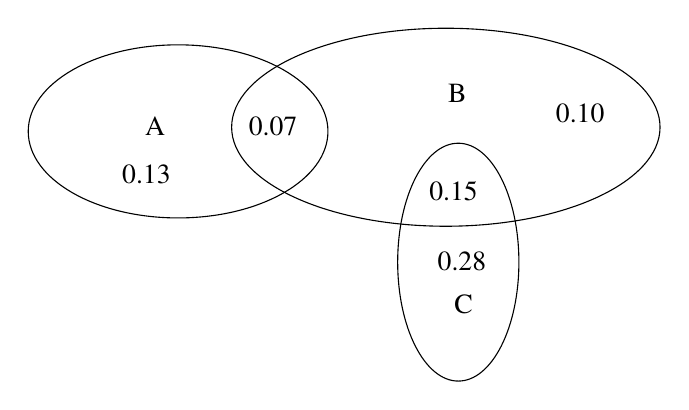
\begin{tikzpicture}[x=0.75pt,y=0.75pt,yscale=-1,xscale=1] 
 
\draw   (106,103.3) .. controls (106,80.27) and (138.33,61.6) .. (178.2,61.6) .. controls (218.07,61.6) and (250.4,80.27) .. (250.4,103.3) .. controls (250.4,126.33) and (218.07,145) .. (178.2,145) .. controls (138.33,145) and (106,126.33) .. (106,103.3) -- cycle ; 
\draw   (204,101.3) .. controls (204,74.96) and (250.2,53.6) .. (307.2,53.6) .. controls (364.2,53.6) and (410.4,74.96) .. (410.4,101.3) .. controls (410.4,127.64) and (364.2,149) .. (307.2,149) .. controls (250.2,149) and (204,127.64) .. (204,101.3) -- cycle ; 
\draw   (313.2,109) .. controls (329.33,109) and (342.4,134.65) .. (342.4,166.3) .. controls (342.4,197.95) and (329.33,223.6) .. (313.2,223.6) .. controls (297.07,223.6) and (284,197.95) .. (284,166.3) .. controls (284,134.65) and (297.07,109) .. (313.2,109) -- cycle ; 
 
\draw (161,95) node [anchor=north west][inner sep=0.75pt]   [align=left] {A}; 
\draw (307,79) node [anchor=north west][inner sep=0.75pt]   [align=left] {B}; 
\draw (310,181) node [anchor=north west][inner sep=0.75pt]   [align=left] {C}; 
\draw (150,118) node [anchor=north west][inner sep=0.75pt]   [align=left] {0.13}; 
\draw (211,95) node [anchor=north west][inner sep=0.75pt]   [align=left] {0.07}; 
\draw (298,126) node [anchor=north west][inner sep=0.75pt]   [align=left] {0.15}; 
\draw (359,89) node [anchor=north west][inner sep=0.75pt]   [align=left] {0.10}; 
\draw (302,160) node [anchor=north west][inner sep=0.75pt]   [align=left] {0.28\\}; 
 
 
\end{tikzpicture}

		\caption {generated by Latextikz}
		\label{fig:exemplar/11/16/3/11}
	\end{figure}
		\solution
		\iffalse
\documentclass[journal,11pt,onecolumn]{IEEEtran}
\usepackage{setspace}
\usepackage{gensymb}
\singlespacing
\usepackage[cmex10]{amsmath}
\usepackage{amsthm}
\usepackage{mathrsfs}
\usepackage{txfonts}
\usepackage{stfloats}
\usepackage{bm}
\usepackage{cite}
\usepackage{cases}
\usepackage{subfig}
\usepackage{longtable}
\usepackage{multirow}
\usepackage{enumitem}
\usepackage{mathtools}
\usepackage{tikz}
\usepackage{circuitikz}
\usepackage{verbatim}
\usepackage[breaklinks=true]{hyperref}
\usepackage{tkz-euclide} % loads  TikZ and tkz-base
\usepackage{listings}
\usepackage{color}    
\usepackage{array}    
\usepackage{longtable}
\usepackage{calc}     
\usepackage{multirow} 
\usepackage{hhline}   
\usepackage{ifthen}   
\usepackage{lscape}     
\usepackage{chngcntr}
\usepackage{float}
\DeclareMathOperator*{\Res}{Res}
\renewcommand\thesection{\arabic{section}}
\renewcommand\thesubsection{\thesection.\arabic{subsection}}
\renewcommand\thesubsubsection{\thesubsection.\arabic{subsubsection}}

\renewcommand\thesectiondis{\arabic{section}}
\renewcommand\thesubsectiondis{\thesectiondis.\arabic{subsection}}
\renewcommand\thesubsubsectiondis{\thesubsectiondis.\arabic{subsubsection}}
\renewcommand\thetable{\arabic{table}}
% correct bad hyphenation here
\hyphenation{op-tical net-works semi-conduc-tor}
\def\inputGnumericTable{}                                 %%

\lstset{
%language=C,
frame=single, 
breaklines=true,
columns=fullflexible
}
%\lstset{
%language=tex,
%frame=single, 
%breaklines=true
%}

\title{Assignment}
\author{Barath surya M | EE22BTECH11014}
\begin{document}
\newtheorem{theorem}{Theorem}[section]
\newtheorem{problem}{Problem}
\newtheorem{proposition}{Proposition}[section]
\newtheorem{lemma}{Lemma}[section]
\newtheorem{corollary}[theorem]{Corollary}
\newtheorem{example}{Example}[section]
\newtheorem{definition}[problem]{Definition}
\newcommand{\BEQA}{\begin{eqnarray}}
\newcommand{\EEQA}{\end{eqnarray}}
\newcommand{\define}{\stackrel{\triangle}{=}}
\bibliographystyle{IEEEtran}
\providecommand{\mbf}{\mathbf}
\providecommand{\pr}[1]{\ensuremath{\Pr\left(#1\right)}}
\providecommand{\qfunc}[1]{\ensuremath{Q\left(#1\right)}}
\providecommand{\sbrak}[1]{\ensuremath{{}\left[#1\right]}}
\providecommand{\lsbrak}[1]{\ensuremath{{}\left[#1\right.}}
\providecommand{\rsbrak}[1]{\ensuremath{{}\left.#1\right]}}
\providecommand{\brak}[1]{\ensuremath{\left(#1\right)}}
\providecommand{\lbrak}[1]{\ensuremath{\left(#1\right.}}
\providecommand{\rbrak}[1]{\ensuremath{\left.#1\right)}}
\providecommand{\cbrak}[1]{\ensuremath{\left\{#1\right\}}}
\providecommand{\lcbrak}[1]{\ensuremath{\left\{#1\right.}}
\providecommand{\rcbrak}[1]{\ensuremath{\left.#1\right\}}}
\theoremstyle{remark}
\newtheorem{rem}{Remark}
\newcommand{\sgn}{\mathop{\mathrm{sgn}}}
\providecommand{\abs}[1]{\left\vert#1\right\vert}
\providecommand{\res}[1]{\Res\displaylimits_{#1}} 
\providecommand{\norm}[1]{\left\lVert#1\right\rVert}
\providecommand{\mtx}[1]{\mathbf{#1}}
\providecommand{\mean}[1]{E\left[ #1 \right]}
\providecommand{\fourier}{\overset{\mathcal{F}}{ \rightleftharpoons}}
\providecommand{\system}[1]{\overset{\mathcal{#1}}{ \longleftrightarrow}}
\newcommand{\solution}{\noindent \textbf{Solution: }}
\newcommand{\cosec}{\,\text{cosec}\,}
\providecommand{\dec}[2]{\ensuremath{\overset{#1}{\underset{#2}{\gtrless}}}}
\newcommand{\myvec}[1]{\ensuremath{\begin{pmatrix}#1\end{pmatrix}}}
\newcommand{\mydet}[1]{\ensuremath{\begin{vmatrix}#1\end{vmatrix}}}
\let\vec\mathbf
\def\putbox#1#2#3{\makebox[0in][l]{\makebox[#1][l]{}\raisebox{\baselineskip}[0in][0in]{\raisebox{#2}[0in][0in]{#3}}}}
     \def\rightbox#1{\makebox[0in][r]{#1}}
     \def\centbox#1{\makebox[0in]{#1}}
     \def\topbox#1{\raisebox{-\baselineskip}[0in][0in]{#1}}
     \def\midbox#1{\raisebox{-0.5\baselineskip}[0in][0in]{#1}}
\maketitle
\vspace{3cm}
Question 11.16.3.11\\
The accompanying venn diagram shows three events, A, B and C, and also the probabilities of the various intersections (for instance, $\pr{AB}=0.7$. Determine 
\begin{enumerate}
	\item \pr{A}
	\item \pr{BC'}
	\item \pr{A+B}
	\item \pr{AB'}
	\item \pr{BC}
	\item \text{Probability of exactly one of the three occurs}
\end{enumerate}
\begin{figure}[h!]
	\centering
	\tikzset{every picture/.style={line width=0.75pt}}   
 
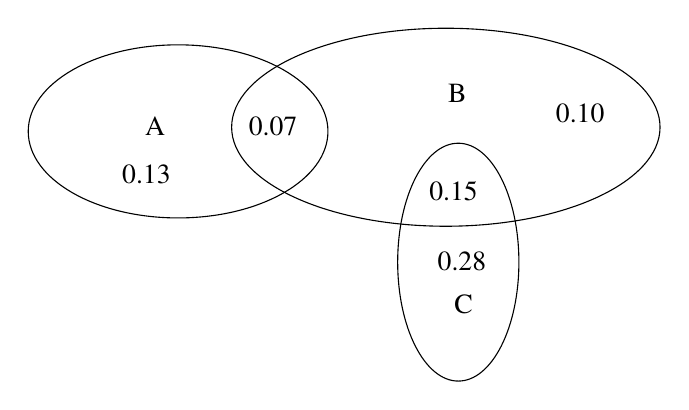
\begin{tikzpicture}[x=0.75pt,y=0.75pt,yscale=-1,xscale=1] 
 
\draw   (106,103.3) .. controls (106,80.27) and (138.33,61.6) .. (178.2,61.6) .. controls (218.07,61.6) and (250.4,80.27) .. (250.4,103.3) .. controls (250.4,126.33) and (218.07,145) .. (178.2,145) .. controls (138.33,145) and (106,126.33) .. (106,103.3) -- cycle ; 
\draw   (204,101.3) .. controls (204,74.96) and (250.2,53.6) .. (307.2,53.6) .. controls (364.2,53.6) and (410.4,74.96) .. (410.4,101.3) .. controls (410.4,127.64) and (364.2,149) .. (307.2,149) .. controls (250.2,149) and (204,127.64) .. (204,101.3) -- cycle ; 
\draw   (313.2,109) .. controls (329.33,109) and (342.4,134.65) .. (342.4,166.3) .. controls (342.4,197.95) and (329.33,223.6) .. (313.2,223.6) .. controls (297.07,223.6) and (284,197.95) .. (284,166.3) .. controls (284,134.65) and (297.07,109) .. (313.2,109) -- cycle ; 
 
\draw (161,95) node [anchor=north west][inner sep=0.75pt]   [align=left] {A}; 
\draw (307,79) node [anchor=north west][inner sep=0.75pt]   [align=left] {B}; 
\draw (310,181) node [anchor=north west][inner sep=0.75pt]   [align=left] {C}; 
\draw (150,118) node [anchor=north west][inner sep=0.75pt]   [align=left] {0.13}; 
\draw (211,95) node [anchor=north west][inner sep=0.75pt]   [align=left] {0.07}; 
\draw (298,126) node [anchor=north west][inner sep=0.75pt]   [align=left] {0.15}; 
\draw (359,89) node [anchor=north west][inner sep=0.75pt]   [align=left] {0.10}; 
\draw (302,160) node [anchor=north west][inner sep=0.75pt]   [align=left] {0.28\\}; 
 
 
\end{tikzpicture}

	\caption {generated by Latextikz}
	\label{fig:exemplar/11/16/3/11}
\end{figure}
\solution
\fi
Given:\\
From \figref{fig:exemplar/11/16/3/11}
\begin{align}
\pr{AB}=0.07\\
\pr{AB'}=0.13\\
\pr{BC}=0.15\\
\pr{BA'C'}=0.10\\
\pr{CB'}=0.28
\end{align}
\begin{enumerate}
\item \begin{align}
	\pr{A}&= 0.13+0.07\\
	&=0.2
	\end{align}
\item \begin{align}
	\pr{BC'} &=0.07+0.10+0.15-0.15\\
	&=0.17
\end{align}
\item \begin{align}
	\pr{A+B}&= \pr{A}+\pr{B} -\pr{AB}\\
	&=0.20+\brak{0.07+0.10+0.15}-0.07\\
	&=0.45
\end{align} 
\item \begin{align}
	\pr{AB'}&=0.20-0.07\\
	&=0.13
\end{align}
\item \begin{align}
	\pr{BC}&=0.15
\end{align} 
\item \begin{align}
	\pr{\text{AB'}} +\pr{CB'}+\pr{BA'C'} &= 0.13+0.10+0.28\\
	&=0.51
\end{align} 
\end{enumerate}


 

	\item One urn contains two black balls (labelled B1 and B2) and one white ball. A
	second urn contains one black ball and two white balls (labelled W1 and W2).
	Suppose the following experiment is performed. One of the two urns is chosen
	at random. Next a ball is randomly chosen from the urn. Then a second ball is
	chosen at random from the same urn without replacing the first ball.
	
	\begin{enumerate}
	\item What is the probability that two black balls are chosen?
	
	\item What is the probability that two balls of opposite colour are chosen?
	\end{enumerate}
	\solution
	\iffalse
\let\negmedspace\undefined
\let\negthickspace\undefined
\documentclass[journal,12pt,twocolumn]{IEEEtran}
\usepackage{cite}
\usepackage{amsmath,amssymb,amsfonts,amsthm}
\usepackage{algorithmic}
\usepackage{graphicx}
\usepackage{textcomp}
\usepackage{xcolor}
\usepackage{txfonts}
\usepackage{listings}
%\usepackage{enumitem}
\usepackage{mathtools}
\usepackage{gensymb}
\usepackage[breaklinks=true]{hyperref}
\usepackage{tkz-euclide} % loads  TikZ and tkz-base
\usepackage{listings}
\usepackage[inline]{enumitem}
\DeclareMathOperator*{\Res}{Res}
\renewcommand\thesection{\arabic{section}}
\renewcommand\thesubsection{\thesection.\arabic{subsection}}
\renewcommand\thesubsubsection{\thesubsection.\arabic{subsubsection}}


\def\inputGnumericTable{}

\usepackage[latin1]{inputenc}                                 
\usepackage{color}                                            
\usepackage{array}                                            
\usepackage{longtable}                                        
\usepackage{calc}                                             
\usepackage{multirow}                                         
\usepackage{hhline}                                           
\usepackage{ifthen}
\usepackage{caption} 
\captionsetup[table]{skip=3pt}  
\providecommand{\pr}[1]{\ensuremath{\Pr\left(#1\right)}}
\providecommand{\cbrak}[1]{\ensuremath{\left\{#1\right\}}}

\renewcommand\thesectiondis{\arabic{section}}
\renewcommand\thesubsectiondis{\thesectiondis.\arabic{subsection}}
\renewcommand\thesubsubsectiondis{\thesubsectiondis.\arabic{subsubsection}}

\def\inputGnumericTable{}                                 %%

\lstset{
frame=single, 
breaklines=true,
columns=fullflexible
}

\begin{document}

\newtheorem{theorem}{Theorem}[section]
\newtheorem{problem}{Problem}
\newtheorem{proposition}{Proposition}[section]
\newtheorem{lemma}{Lemma}[section]
\newtheorem{corollary}[theorem]{Corollary}
\newtheorem{example}{Example}[section]
\newtheorem{definition}[problem]{Definition}
\newcommand{\BEQA}{\begin{eqnarray}}
\newcommand{\EEQA}{\end{eqnarray}}
\newcommand{\define}{\stackrel{\triangle}{=}}
\newcommand{\xor}{\oplus}
\bibliographystyle{IEEEtran}

\providecommand{\mbf}{\mathbf}
\providecommand{\pr}[1]{\ensuremath{\Pr\left(#1\right)}}
\providecommand{\qfunc}[1]{\ensuremath{Q\left(#1\right)}}
\providecommand{\sbrak}[1]{\ensuremath{{}\left[#1\right]}}
\providecommand{\lsbrak}[1]{\ensuremath{{}\left[#1\right.}}
\providecommand{\rsbrak}[1]{\ensuremath{{}\left.#1\right]}}
\providecommand{\brak}[1]{\ensuremath{\left(#1\right)}}
\providecommand{\lbrak}[1]{\ensuremath{\left(#1\right.}}
\providecommand{\rbrak}[1]{\ensuremath{\left.#1\right)}}
\providecommand{\cbrak}[1]{\ensuremath{\left\{#1\right\}}}
\providecommand{\lcbrak}[1]{\ensuremath{\left\{#1\right.}}
\providecommand{\rcbrak}[1]{\ensuremath{\left.#1\right\}}}
\theoremstyle{remark}
\newtheorem{rem}{Remark}
\newcommand{\sgn}{\mathop{\mathrm{sgn}}}

\newcommand{\solution}{\noindent \textbf{Solution: }}
\newcommand{\cosec}{\,\text{cosec}\,}
\providecommand{\dec}[2]{\ensuremath{\overset{#1}{\underset{#2}{\gtrless}}}}
\newcommand{\myvec}[1]{\ensuremath{\begin{pmatrix}#1\end{pmatrix}}}
\newcommand{\mydet}[1]{\ensuremath{\begin{vmatrix}#1\end{vmatrix}}}

\let\vec\mathbf


\vspace{3cm}

\title{
  

  Assignment -2 in \LaTeX
    
  }
  \author{ Muzaan Mohammed Faizel A P\\
  EE22BTECH11036
  }	
% make the title area
\maketitle
\newpage
\bigskip
\renewcommand{\thefigure}{\theenumi}
\renewcommand{\thetable}{\theenumi}
\renewcommand{\thetable}{\arabic{table}}  
\textbf{11.16.3.12}:
One urn contains two black balls (labelled B1 and B2) and one white ball. A
second urn contains one black ball and two white balls (labelled W1 and W2).
Suppose the following experiment is performed. One of the two urns is chosen
at random. Next a ball is randomly chosen from the urn. Then a second ball is
chosen at random from the same urn without replacing the first ball.

\begin{enumerate}
	
\item What is the probability that two black balls are chosen?

\item What is the probability that two balls of opposite colour are chosen?
\end{enumerate}


%Answer
\solution
\fi
Let $X$ be a Bernoulli random variable
    \begin{align} 
    X=
    \begin{cases}
      0, & \text{ Urn 1  }\\
      1, & \text{Urn 2}
    \end{cases}
\end{align}
  Since both events are equally likely
  \begin{align}
  \pr{X=0} &= \pr{X=1}\\
         &=\frac{1}{2}
  \end{align}
  Let $Y_i$ be a random variable to denote the  turn
  \begin{align}
    Y_i=
    \begin{cases}
      0, & \text{Black ball }\\
      1, & \text{White ball }
    \end{cases}
  \end{align}
$Y_1$ denotes the first ball and $Y_2$ denotes the second ball.
\begin{table}[ht!]
		\centering
		%%%%%%%%%%%%%%%%%%%%%%%%%%%%%%%%%%%%%%%%%%%%%%%%%%%%%%%%%%%%%%%%%%%%%%
%%                                                                  %%
%%  This is a LaTeX2e table fragment exported from Gnumeric.        %%
%%                                                                  %%
%%%%%%%%%%%%%%%%%%%%%%%%%%%%%%%%%%%%%%%%%%%%%%%%%%%%%%%%%%%%%%%%%%%%%%

\begin{center}
\begin{tabular}{|c|c|c|}
\hline
\textbf{RV}& \textbf{Values} & \textbf{Description} \\ \hline
$X$		   & 	$\{0,1\}$	&  1st draw - 0: Red, 1: Black\\ \hline
$Y$ 		   & 	$\{0,1\}$	&  2nd draw - 0: Red, 1: Black\\ \hline
\end{tabular}
\end{center}

		\caption{Random variables for each ball}
		\label{tab:table1exemp}	
	\end{table}
\begin{enumerate}

\item 
\begin{align}
E &= \brak{Y_1+Y_2}^\prime  \\
&= Y_1^\prime Y_2^\prime
\end{align}
Required Probability:
\begin{align}  
&\pr{Y_1^\prime Y_2^\prime}=\pr{Y_1^\prime Y_2^\prime | X^\prime}\pr{X^\prime} \\ 
&= \frac{2}{3}\times\frac{1}{2}\times\frac{1}{2} \\ 
&= 1/6 
\end{align}
Therefore,
\begin{align}
\pr{E} = \frac{1}{6} 
\end{align}
\item 
\begin{align}
E&= Y_1 Y_2^\prime + Y_1^\prime Y_2
\end{align}
Required Probability : 
\begin{align}
&\pr{Y_1 Y_2^\prime + Y_1^\prime Y_2}=\pr{Y_1 Y_2^\prime} + \pr{Y_1^\prime Y_2} \\
&=\brak{\frac{1}{3}\times\frac{1}{2} + \frac{2}{3}\times\frac{1}{2}\times\frac{1}{2}}\times 2 \\
&=\frac{2}{3}
\end{align}
Therefore,
\begin{align}
\pr{E} &= \frac{2}{3}
\end{align}
\end{enumerate}


  
\item Events E and F are such that P(not E or not F) = 0.25, State whether E and F are
mutually exclusive.
\iffalse
\let\negmedspace\undefined
\let\negthickspace\undefined
\documentclass[article]{IEEEtran}
       \def\inputGnumericTable{}                                 %%
\usepackage{cite}
\usepackage{amsmath,amssymb,amsfonts,amsthm}
\usepackage{algorithmic}
\usepackage{graphicx}
\usepackage{textcomp}
\usepackage{xcolor}
\usepackage{txfonts}
\usepackage{listings}
\usepackage{enumitem}
\usepackage{mathtools}
\usepackage{gensymb}
\usepackage[breaklinks=true]{hyperref}
\usepackage{tkz-euclide} % loads  TikZ and tkz-base
\usepackage{listings}
%
%\usepackage{setspace}
%\usepackage{gensymb}
%\doublespacing
%\singlespacing

%\usepackage{graphicx}
%\usepackage{amssymb}
%\usepackage{relsize}
%\usepackage[cmex10]{amsmath}
%\usepackage{amsthm}
%\interdisplaylinepenalty=2500
%\savesymbol{iint}
%\usepackage{txfonts}
%\restoresymbol{TXF}{iint}
%\usepackage{wasysym}
%\usepackage{amsthm}
%\usepackage{iithtlc}
%\usepackage{mathrsfs}
%\usepackage{txfonts}
%\usepackage{stfloats}
%\usepackage{bm}
%\usepackage{cite}
%\usepackage{cases}
%\usepackage{subfig}
%\usepackage{xtab}
%\usepackage{longtable}
%\usepackage{multirow}
%\usepackage{algorithm}
%\usepackage{algpseudocode}
%\usepackage{enumitem}
%\usepackage{mathtools}
%\usepackage{tikz}
%\usepackage{circuitikz}
%\usepackage{verbatim}
%\usepackage{tfrupee}
%\usepackage{stmaryrd}
%\usetkzobj{all}
    \usepackage{color}                                            %%
    \usepackage{array}                                            %%
    \usepackage{longtable}                                        %%
    \usepackage{calc}                                             %%
    \usepackage{multirow}                                         %%
    \usepackage{hhline}                                           %%
    \usepackage{ifthen}                                           %%
 %optionally (for landscape tables embedded in another document): %%
    \usepackage{lscape}     
%\usepackage{multicol}
%\usepackage{chngcntr}
%\usepackage{enumerate}

%\usepackage{wasysym}
%\documentclass[conference]{IEEEtran}
%\IEEEoverridecommandlockouts
% The preceding line is only needed to identify funding in the first footnote. If that is unneeded, please comment it out.

\newtheorem{theorem}{Theorem}[section]
\newtheorem{problem}{Problem}
\newtheorem{proposition}{Proposition}[section]
\newtheorem{lemma}{Lemma}[section]
\newtheorem{corollary}[theorem]{Corollary}
\newtheorem{example}{Example}[section]
\newtheorem{definition}[problem]{Definition}
%\newtheorem{thm}{Theorem}[section] 
%\newtheorem{defn}[thm]{Definition}
%\newtheorem{algorithm}{Algorithm}[section]
%\newtheorem{cor}{Corollary}
\newcommand{\BEQA}{\begin{eqnarray}}
\newcommand{\EEQA}{\end{eqnarray}}
\newcommand{\define}{\stackrel{\triangle}{=}}
\theoremstyle{remark}
\newtheorem{rem}{Remark}

\begin{document}
\providecommand{\pr}[1]{\ensuremath{\Pr\left(#1\right)}}
\providecommand{\prt}[2]{\ensuremath{p_{#1}^{\left(#2\right)} }}        % own macro for this question
\providecommand{\qfunc}[1]{\ensuremath{Q\left(#1\right)}}
\providecommand{\sbrak}[1]{\ensuremath{{}\left[#1\right]}}
\providecommand{\lsbrak}[1]{\ensuremath{{}\left[#1\right.}}
\providecommand{\rsbrak}[1]{\ensuremath{{}\left.#1\right]}}
\providecommand{\brak}[1]{\ensuremath{\left(#1\right)}}
\providecommand{\lbrak}[1]{\ensuremath{\left(#1\right.}}
\providecommand{\rbrak}[1]{\ensuremath{\left.#1\right)}}
\providecommand{\cbrak}[1]{\ensuremath{\left\{#1\right\}}}
\providecommand{\lcbrak}[1]{\ensuremath{\left\{#1\right.}}
\providecommand{\rcbrak}[1]{\ensuremath{\left.#1\right\}}}
\newcommand{\sgn}{\mathop{\mathrm{sgn}}}
\providecommand{\abs}[1]{\left\vert#1\right\vert}
\providecommand{\res}[1]{\Res\displaylimits_{#1}} 
\providecommand{\norm}[1]{\left\lVert#1\right\rVert}
%\providecommand{\norm}[1]{\lVert#1\rVert}
\providecommand{\mtx}[1]{\mathbf{#1}}
\providecommand{\mean}[1]{E\left[ #1 \right]}
\providecommand{\cond}[2]{#1\middle|#2}
\providecommand{\fourier}{\overset{\mathcal{F}}{ \rightleftharpoons}}
\newenvironment{amatrix}[1]{%
  \left(\begin{array}{@{}*{#1}{c}|c@{}}
}{%
  \end{array}\right)
}
%\providecommand{\hilbert}{\overset{\mathcal{H}}{ \rightleftharpoons}}
%\providecommand{\system}{\overset{\mathcal{H}}{ \longleftrightarrow}}
	%\newcommand{\solution}[2]{\textbf{Solution:}{#1}}
\newcommand{\solution}{\noindent \textbf{Solution: }}
\newcommand{\cosec}{\,\text{cosec}\,}
\providecommand{\dec}[2]{\ensuremath{\overset{#1}{\underset{#2}{\gtrless}}}}
\newcommand{\myvec}[1]{\ensuremath{\begin{pmatrix}#1\end{pmatrix}}}
\newcommand{\mydet}[1]{\ensuremath{\begin{vmatrix}#1\end{vmatrix}}}
\newcommand{\myaugvec}[2]{\ensuremath{\begin{amatrix}{#1}#2\end{amatrix}}}
\providecommand{\rank}{\text{rank}}
\providecommand{\pr}[1]{\ensuremath{\Pr\left(#1\right)}}
\providecommand{\qfunc}[1]{\ensuremath{Q\left(#1\right)}}
	\newcommand*{\permcomb}[4][0mu]{{{}^{#3}\mkern#1#2_{#4}}}
\newcommand*{\perm}[1][-3mu]{\permcomb[#1]{P}}
\newcommand*{\comb}[1][-1mu]{\permcomb[#1]{C}}
\providecommand{\qfunc}[1]{\ensuremath{Q\left(#1\right)}}
\providecommand{\gauss}[2]{\mathcal{N}\ensuremath{\left(#1,#2\right)}}
\providecommand{\diff}[2]{\ensuremath{\frac{d{#1}}{d{#2}}}}
\providecommand{\myceil}[1]{\left \lceil #1 \right \rceil }
\newcommand\figref{Fig.~\ref}
\newcommand\tabref{Table~\ref}
\newcommand{\sinc}{\,\text{sinc}\,}
\newcommand{\rect}{\,\text{rect}\,}
%%
%	%\newcommand{\solution}[2]{\textbf{Solution:}{#1}}
%\newcommand{\solution}{\noindent \textbf{Solution: }}
%\newcommand{\cosec}{\,\text{cosec}\,}
%\numberwithin{equation}{section}
%\numberwithin{equation}{subsection}
%\numberwithin{problem}{section}
%\numberwithin{definition}{section}
%\makeatletter
%\@addtoreset{figure}{problem}
%\makeatother

%\let\StandardTheFigure\thefigure
\let\vec\mathbf

\bibliographystyle{IEEEtran}
\title{
%	\logo{
Assignment
%	}
}
\author{ Karthikeya hanu prakash kanithi (EE22BTECH11026)}
\maketitle

\vspace{3cm}
Question : Three dice are thrown at the sametime. Find the probability of getting three
two’s, if it is known that the sum of the numbers on the dice was six.
\fi
\\\solution 
Let $X_1, X_2, X_3$ be Bernoulli Random Variables as defined in  \autoref{tab:exemplar/12/13/3/14},
\begin{table}[h]
	\centering
	\input{exemplar/12/13/3/14/tables/Table2.tex}
	\caption{Random variable $X_i$ declaration $\forall i \in {1,2,3}$.}
        \label{tab:exemplar/12/13/3/14}
\end{table}
\\We need to find the value of
\begin{align}
\pr{X_1=2,X_2=2,X_3=2|X_1+X_2+X_3=6}
\end{align}
\\The pmf's of the random variables are as follows:
\begin{equation}
    p_{X_1}(k) = \label{eq:12/13/3/14}
    \begin{cases}
        \frac{1}{6} &  x \in \{1,2,3,4,5,6\} \\
        0 &  \text{otherwise}
    \end{cases}
\end{equation}
Now, If 
\begin{align}
X=X_1+X_2+X_3
\end{align}
Then
\begin{align}
      M_{X}(z)&=\prod_{i=1}^{3}M_{X_i}(z)\\
      &= \prod_{i=1}^{3}\left(\sum_{k=1}^{6} \frac{z^{-k}}{6}\right) \label{eq:12/13/3/14/3}\\
      &= \frac{z^{-3}}{216} + \frac{3z^{-4}}{216} + \frac{6z^{-5}}{216} + \frac{10z^{-6}}{216} + \ldots 
\end{align}
From \eqref{eq:12/13/3/14}, When all the three die's roll 2, then thier sum will be 6. So, 
\begin{align}
&\pr{X_1=X_2=X_3=2 ,\ X_1+X_2+X_3=6} \label{eq:12/13/3/14/4} \\ 
&= p_{X_1}(2) p_{X_2}(2) p_{X_3}(2)
= \left(\frac{1}{6}\right)^3
= \frac{1}{216}
\end{align}
From \eqref{eq:12/13/3/14/3}, the probability that the sum of all three die's is 6 is,
\begin{align}
\pr{X_1+X_2+X_3=6} &= \frac{10}{216} \label{eq:12/13/3/14/5}
\end{align}
From \eqref{eq:12/13/3/14/4} and \eqref{eq:12/13/3/14/5}, the probability of getting three two’s, if it is known that the sum of the numbers on the dice was six will be
\begin{align}
&\pr{X_1=2,X_2=2,X_3=2|X_1+X_2+X_3=6} \\ 
&= \frac{\pr{X_1=X_2=X_3=2 ,\ X_1+X_2+X_3=6}}{\pr{X_1+X_2+X_3=6}}\\
&= \frac{\frac{1}{216}}{\frac{10}{216}}
=\frac{1}{10}
\end{align}






















\item Suppose an integer from 1 through 1000 is chosen at random, find the probability that the integer is a multiple of 2 or a multiple of 9.
\iffalse
\let\negmedspace\undefined
\let\negthickspace\undefined
\documentclass[journal,12pt,onecolumn]{IEEEtran}
\usepackage{cite}
\usepackage{amsmath,amssymb,amsfonts,amsthm}
\usepackage{algorithmic}
\usepackage{graphicx}
\usepackage{textcomp}
\usepackage{xcolor}
\usepackage{txfonts}
\usepackage{listings}
\usepackage{enumitem}
\usepackage{mathtools}
\usepackage{gensymb}
\usepackage{comment}
\usepackage[breaklinks=true]{hyperref}
\usepackage{tkz-euclide} 
\usepackage{listings}
\usepackage{gvv}                                        
\def\inputGnumericTable{}                                 
\usepackage[latin1]{inputenc}                                
\usepackage{color}                                            
\usepackage{array}                                            
\usepackage{longtable}                                       
\usepackage{calc}                                             
\usepackage{multirow}                                         
\usepackage{hhline}                                           
\usepackage{ifthen}                                           
\usepackage{lscape}

\newtheorem{theorem}{Theorem}[section]
\newtheorem{problem}{Problem}
\newtheorem{proposition}{Proposition}[section]
\newtheorem{lemma}{Lemma}[section]
\newtheorem{corollary}[theorem]{Corollary}
\newtheorem{example}{Example}[section]
\newtheorem{definition}[problem]{Definition}
\newcommand{\BEQA}{\begin{eqnarray}}
\newcommand{\EEQA}{\end{eqnarray}}
\newcommand{\define}{\stackrel{\triangle}{=}}
\theoremstyle{remark}
\newtheorem{rem}{Remark}
\begin{document}

\bibliographystyle{IEEEtran}
\vspace{3cm}


\title{Question 12.13.3.18}
\author{EE22BTECH11051}

\maketitle
\vspace{3cm}

\textbf{Question:} A box has 5 blue and 4 red balls. One ball is drawn at random and not replaced.
Its colour is also not noted. Then another ball is drawn at random. What is the
probability of second ball being blue?

\textbf{Solution:} \\
\fi
Let X and Y denote the random variables for the first and second draw respectively as follows:
\begin{table}[h]
    \centering
    %%%%%%%%%%%%%%%%%%%%%%%%%%%%%%%%%%%%%%%%%%%%%%%%%%%%%%%%%%%%%%%%%%%%%%
%%                                                                  %%
%%  This is a LaTeX2e table fragment exported from Gnumeric.        %%
%%                                                                  %%
%%%%%%%%%%%%%%%%%%%%%%%%%%%%%%%%%%%%%%%%%%%%%%%%%%%%%%%%%%%%%%%%%%%%%%

\begin{center}
    \begin{tabular}{|c|c|c|}
    \hline
    \textbf{RV}& \textbf{Values} & \textbf{Description} \\ \hline
    $X$		   & 	$\{0,1\}$	&  1st draw :- 0: blue, 1: red\\ \hline
    $Y$ 		   & 	$\{0,1\}$	&  2nd draw :- 0: blue, 1: red\\ \hline
    \end{tabular}
    \end{center}
    \caption{Random Variables}
    \label{12.13.3.8_table_1}
    \end{table}
\\
The probabilities are given as:
\begin{align}
    \pr{X = 0} = \frac{5}{9}\\
    \pr{X = 1} = \frac{4}{9}
\end{align}
\begin{align}
    \pr{Y = 0 | X = 0} = \frac{\pr{Y = 0,X = 0}}{\pr{X = 0}} = \frac{1}{2}\\
    \pr{Y = 0 | X = 1} = \frac{\pr{Y = 0,X = 1}}{\pr{X = 1}} = \frac{5}{8}
\end{align}
    \\
The probability of the second ball beign drawn being blue is given as:
\begin{align}
\pr{Y = 0} &= \pr{X = 0}\pr{Y = 0 | X = 0} + \pr{X = 1}\pr{Y = 0 | X = 1}\\
           &= {\frac{5}{9}}\times{\frac{1}{2}} + {\frac{4}{9}}\times{{\frac{5}{8}}}\\
           &= \frac{5}{9}
\end{align}

\item The probability that at least one of the events A and B occurs is 0.6. If A and B occur simultaneously with probability 0.2, then $\pr{A^\prime}+\pr{B^\prime} $is\\
\begin{enumerate}
\item 0.4\\
\item 0.8\\
\item 1.2\\
\item 1.6\\
\end{enumerate}
\solution \\
\iffalse
\let\negmedspace\undefined
\let\negthickspace\undefined
\documentclass[journal,12pt,onecolumn]{IEEEtran}
\usepackage{cite}
\usepackage{amsmath,amssymb,amsfonts,amsthm}
\usepackage{algorithmic}
\usepackage{graphicx}
\usepackage{textcomp}
\usepackage{xcolor}
\usepackage{txfonts}
\usepackage{listings}
\usepackage{enumitem}
\usepackage{mathtools}
\usepackage{gensymb}
\usepackage[breaklinks=true]{hyperref}
\usepackage{tkz-euclide} % loads  TikZ and tkz-base
\usepackage{listings}



\newtheorem{theorem}{Theorem}[section]
\newtheorem{problem}{Problem}
\newtheorem{proposition}{Proposition}[section]
\newtheorem{lemma}{Lemma}[section]
\newtheorem{corollary}[theorem]{Corollary}
\newtheorem{example}{Example}[section]
\newtheorem{definition}[problem]{Definition}
%\newtheorem{thm}{Theorem}[section] 
%\newtheorem{defn}[thm]{Definition}
%\newtheorem{algorithm}{Algorithm}[section]
%\newtheorem{cor}{Corollary}
\newcommand{\BEQA}{\begin{eqnarray}}
\newcommand{\EEQA}{\end{eqnarray}}
\newcommand{\define}{\stackrel{\triangle}{=}}
\theoremstyle{remark}
\newtheorem{rem}{Remark}
%\bibliographystyle{ieeetr}
\begin{document}
%
\providecommand{\pr}[1]{\ensuremath{\Pr\left(#1\right)}}
\providecommand{\prt}[2]{\ensuremath{p_{#1}^{\left(#2\right)} }}        % own macro for this question
\providecommand{\qfunc}[1]{\ensuremath{Q\left(#1\right)}}
\providecommand{\sbrak}[1]{\ensuremath{{}\left[#1\right]}}
\providecommand{\lsbrak}[1]{\ensuremath{{}\left[#1\right.}}
\providecommand{\rsbrak}[1]{\ensuremath{{}\left.#1\right]}}
\providecommand{\brak}[1]{\ensuremath{\left(#1\right)}}
\providecommand{\lbrak}[1]{\ensuremath{\left(#1\right.}}
\providecommand{\rbrak}[1]{\ensuremath{\left.#1\right)}}
\providecommand{\cbrak}[1]{\ensuremath{\left\{#1\right\}}}
\providecommand{\lcbrak}[1]{\ensuremath{\left\{#1\right.}}
\providecommand{\rcbrak}[1]{\ensuremath{\left.#1\right\}}}
\newcommand{\sgn}{\mathop{\mathrm{sgn}}}
\providecommand{\abs}[1]{\left\vert#1\right\vert}
\providecommand{\res}[1]{\Res\displaylimits_{#1}} 
\providecommand{\norm}[1]{\left\lVert#1\right\rVert}
%\providecommand{\norm}[1]{\lVert#1\rVert}
\providecommand{\mtx}[1]{\mathbf{#1}}
\providecommand{\mean}[1]{E\left[ #1 \right]}
\providecommand{\cond}[2]{#1\middle|#2}
\providecommand{\fourier}{\overset{\mathcal{F}}{ \rightleftharpoons}}
\newenvironment{amatrix}[1]{%
  \left(\begin{array}{@{}*{#1}{c}|c@{}}
}{%
  \end{array}\right)
}
%\providecommand{\hilbert}{\overset{\mathcal{H}}{ \rightleftharpoons}}
%\providecommand{\system}{\overset{\mathcal{H}}{ \longleftrightarrow}}
	%\newcommand{\solution}[2]{\textbf{Solution:}{#1}}
\newcommand{\solution}{\noindent \textbf{Solution: }}
\newcommand{\cosec}{\,\text{cosec}\,}
\providecommand{\dec}[2]{\ensuremath{\overset{#1}{\underset{#2}{\gtrless}}}}
\newcommand{\myvec}[1]{\ensuremath{\begin{pmatrix}#1\end{pmatrix}}}
\newcommand{\mydet}[1]{\ensuremath{\begin{vmatrix}#1\end{vmatrix}}}
\newcommand{\myaugvec}[2]{\ensuremath{\begin{amatrix}{#1}#2\end{amatrix}}}
\providecommand{\rank}{\text{rank}}
\providecommand{\pr}[1]{\ensuremath{\Pr\left(#1\right)}}
\providecommand{\qfunc}[1]{\ensuremath{Q\left(#1\right)}}
	\newcommand*{\permcomb}[4][0mu]{{{}^{#3}\mkern#1#2_{#4}}}
\newcommand*{\perm}[1][-3mu]{\permcomb[#1]{P}}
\newcommand*{\comb}[1][-1mu]{\permcomb[#1]{C}}
\providecommand{\qfunc}[1]{\ensuremath{Q\left(#1\right)}}
\providecommand{\gauss}[2]{\mathcal{N}\ensuremath{\left(#1,#2\right)}}
\providecommand{\diff}[2]{\ensuremath{\frac{d{#1}}{d{#2}}}}
\providecommand{\myceil}[1]{\left \lceil #1 \right \rceil }
\newcommand\figref{Fig.~\ref}
\newcommand\tabref{Table~\ref}
\newcommand{\sinc}{\,\text{sinc}\,}
\newcommand{\rect}{\,\text{rect}\,}
%%
%	%\newcommand{\solution}[2]{\textbf{Solution:}{#1}}
%\newcommand{\solution}{\noindent \textbf{Solution: }}
%\newcommand{\cosec}{\,\text{cosec}\,}
%\numberwithin{equation}{section}
%\numberwithin{equation}{subsection}
%\numberwithin{problem}{section}
%\numberwithin{definition}{section}
%\makeatletter
%\@addtoreset{figure}{problem}
%\makeatother

%\let\StandardTheFigure\thefigure
\let\vec\mathbf

\bibliographystyle{IEEEtran}


\vspace{3cm}



\bigskip

\renewcommand{\thefigure}{\theenumi}
\renewcommand{\thetable}{\theenumi}
%\renewcommand{\theequation}{\theenumi}
Question:The probability that at least one of the events A and B occurs is 0.6. If A and B occur simultaneously with probability 0.2, then $\pr{A^\prime}+\pr{B^\prime} $is\\
(A) 0.4\\
(B) 0.8\\
(C) 1.2\\
(D) 1.6\\
\solution:
\fi
Given,
\begin{align}
\pr{A+B}=0.6\\
\pr{AB}=0.2
\end{align}
\begin{align}
\pr{A+B}&=\pr{A}+\pr{B}-\pr{AB}\\
0.6&=\pr{A}+\pr{B}-0.2
\end{align}
\begin{align}
\implies \pr{A}+\pr{B}=0.8\\
1 -\pr{ A^\prime}+1-\pr{B^\prime}=0.8\\
\therefore \pr{A^\prime}+\pr{B^\prime}=1.2
\end{align}

\item State whether the statement is True or False.\\
The probability that a person visiting a zoo will see the giraffe is 0.72, the probability that he will see the bears is 0.84 and the probability that he will see both is 0.52.\\
\solution
\\
\iffalse
\let\negmedspace\undefined
\let\negthickspace\undefined
\documentclass[journal,12pt,onecolumn]{IEEEtran}
\usepackage{cite}
\usepackage{amsmath,amssymb,amsfonts,amsthm}
\usepackage{algorithmic}
\usepackage{graphicx}
\usepackage{textcomp}
\usepackage{xcolor}
\usepackage{txfonts}
\usepackage{listings}
\usepackage{enumitem}
\usepackage{mathtools}
\usepackage{gensymb}
\usepackage{comment}
\usepackage[breaklinks=true]{hyperref}
\usepackage{tkz-euclide} 
\usepackage{listings}
\usepackage{gvv}                                        
\def\inputGnumericTable{}                                 
\usepackage[latin1]{inputenc}                                
\usepackage{color}                                            
\usepackage{array}                                            
\usepackage{longtable}                                       
\usepackage{calc}                                             
\usepackage{multirow}                                         
\usepackage{hhline}                                           
\usepackage{ifthen}                                           
\usepackage{lscape}

\newtheorem{theorem}{Theorem}[section]
\newtheorem{problem}{Problem}
\newtheorem{proposition}{Proposition}[section]
\newtheorem{lemma}{Lemma}[section]
\newtheorem{corollary}[theorem]{Corollary}
\newtheorem{example}{Example}[section]
\newtheorem{definition}[problem]{Definition}
\newcommand{\BEQA}{\begin{eqnarray}}
\newcommand{\EEQA}{\end{eqnarray}}
\newcommand{\define}{\stackrel{\triangle}{=}}
\theoremstyle{remark}
\newtheorem{rem}{Remark}
\begin{document}

\bibliographystyle{IEEEtran}
\vspace{3cm}


\title{Question 12.13.3.18}
\author{EE22BTECH11051}

\maketitle
\vspace{3cm}

\textbf{Question:} A box has 5 blue and 4 red balls. One ball is drawn at random and not replaced.
Its colour is also not noted. Then another ball is drawn at random. What is the
probability of second ball being blue?

\textbf{Solution:} \\
\fi
Let X and Y denote the random variables for the first and second draw respectively as follows:
\begin{table}[h]
    \centering
    %%%%%%%%%%%%%%%%%%%%%%%%%%%%%%%%%%%%%%%%%%%%%%%%%%%%%%%%%%%%%%%%%%%%%%
%%                                                                  %%
%%  This is a LaTeX2e table fragment exported from Gnumeric.        %%
%%                                                                  %%
%%%%%%%%%%%%%%%%%%%%%%%%%%%%%%%%%%%%%%%%%%%%%%%%%%%%%%%%%%%%%%%%%%%%%%

\begin{center}
    \begin{tabular}{|c|c|c|}
    \hline
    \textbf{RV}& \textbf{Values} & \textbf{Description} \\ \hline
    $X$		   & 	$\{0,1\}$	&  1st draw :- 0: blue, 1: red\\ \hline
    $Y$ 		   & 	$\{0,1\}$	&  2nd draw :- 0: blue, 1: red\\ \hline
    \end{tabular}
    \end{center}
    \caption{Random Variables}
    \label{12.13.3.8_table_1}
    \end{table}
\\
The probabilities are given as:
\begin{align}
    \pr{X = 0} = \frac{5}{9}\\
    \pr{X = 1} = \frac{4}{9}
\end{align}
\begin{align}
    \pr{Y = 0 | X = 0} = \frac{\pr{Y = 0,X = 0}}{\pr{X = 0}} = \frac{1}{2}\\
    \pr{Y = 0 | X = 1} = \frac{\pr{Y = 0,X = 1}}{\pr{X = 1}} = \frac{5}{8}
\end{align}
    \\
The probability of the second ball beign drawn being blue is given as:
\begin{align}
\pr{Y = 0} &= \pr{X = 0}\pr{Y = 0 | X = 0} + \pr{X = 1}\pr{Y = 0 | X = 1}\\
           &= {\frac{5}{9}}\times{\frac{1}{2}} + {\frac{4}{9}}\times{{\frac{5}{8}}}\\
           &= \frac{5}{9}
\end{align}

\item The probability of happening of an event A is 0.5 and that of B is 0.3. If A and B are mutually exclusive events, then the probability of neither A nor B is \underline{\phantom{Blank}}.
	\\	\iffalse
\let\negmedspace\undefined
\let\negthickspace\undefined
\documentclass[journal,12pt,onecolumn]{IEEEtran}
\usepackage{cite}
\usepackage{amsmath,amssymb,amsfonts,amsthm}
\usepackage{algorithmic}
\usepackage{graphicx}
\usepackage{textcomp}
\usepackage{xcolor}
\usepackage{txfonts}
\usepackage{listings}
\usepackage{enumitem}
\usepackage{mathtools}
\usepackage{gensymb}
\usepackage{comment}
\usepackage[breaklinks=true]{hyperref}
\usepackage{tkz-euclide} 
\usepackage{listings}
\usepackage{gvv}                                        
\def\inputGnumericTable{}                                 
\usepackage[latin1]{inputenc}                                
\usepackage{color}                                            
\usepackage{array}                                            
\usepackage{longtable}                                       
\usepackage{calc}                                             
\usepackage{multirow}                                         
\usepackage{hhline}                                           
\usepackage{ifthen}                                           
\usepackage{lscape}

\newtheorem{theorem}{Theorem}[section]
\newtheorem{problem}{Problem}
\newtheorem{proposition}{Proposition}[section]
\newtheorem{lemma}{Lemma}[section]
\newtheorem{corollary}[theorem]{Corollary}
\newtheorem{example}{Example}[section]
\newtheorem{definition}[problem]{Definition}
\newcommand{\BEQA}{\begin{eqnarray}}
\newcommand{\EEQA}{\end{eqnarray}}
\newcommand{\define}{\stackrel{\triangle}{=}}
\theoremstyle{remark}
\newtheorem{rem}{Remark}
\begin{document}

\bibliographystyle{IEEEtran}
\vspace{3cm}


\title{Question 12.13.3.18}
\author{EE22BTECH11051}

\maketitle
\vspace{3cm}

\textbf{Question:} A box has 5 blue and 4 red balls. One ball is drawn at random and not replaced.
Its colour is also not noted. Then another ball is drawn at random. What is the
probability of second ball being blue?

\textbf{Solution:} \\
\fi
Let X and Y denote the random variables for the first and second draw respectively as follows:
\begin{table}[h]
    \centering
    %%%%%%%%%%%%%%%%%%%%%%%%%%%%%%%%%%%%%%%%%%%%%%%%%%%%%%%%%%%%%%%%%%%%%%
%%                                                                  %%
%%  This is a LaTeX2e table fragment exported from Gnumeric.        %%
%%                                                                  %%
%%%%%%%%%%%%%%%%%%%%%%%%%%%%%%%%%%%%%%%%%%%%%%%%%%%%%%%%%%%%%%%%%%%%%%

\begin{center}
    \begin{tabular}{|c|c|c|}
    \hline
    \textbf{RV}& \textbf{Values} & \textbf{Description} \\ \hline
    $X$		   & 	$\{0,1\}$	&  1st draw :- 0: blue, 1: red\\ \hline
    $Y$ 		   & 	$\{0,1\}$	&  2nd draw :- 0: blue, 1: red\\ \hline
    \end{tabular}
    \end{center}
    \caption{Random Variables}
    \label{12.13.3.8_table_1}
    \end{table}
\\
The probabilities are given as:
\begin{align}
    \pr{X = 0} = \frac{5}{9}\\
    \pr{X = 1} = \frac{4}{9}
\end{align}
\begin{align}
    \pr{Y = 0 | X = 0} = \frac{\pr{Y = 0,X = 0}}{\pr{X = 0}} = \frac{1}{2}\\
    \pr{Y = 0 | X = 1} = \frac{\pr{Y = 0,X = 1}}{\pr{X = 1}} = \frac{5}{8}
\end{align}
    \\
The probability of the second ball beign drawn being blue is given as:
\begin{align}
\pr{Y = 0} &= \pr{X = 0}\pr{Y = 0 | X = 0} + \pr{X = 1}\pr{Y = 0 | X = 1}\\
           &= {\frac{5}{9}}\times{\frac{1}{2}} + {\frac{4}{9}}\times{{\frac{5}{8}}}\\
           &= \frac{5}{9}
\end{align}

\item If $A$ and $B$ are mutually exclusive events,then
\begin{enumerate}
\item $\pr{A} \leq\pr{B^\prime}$\\
\item $\pr{A} \geq \pr{B^\prime}$\\
\item $\pr{A} < \pr{B^\prime}$\\
\item $\text{none of these}$
\end{enumerate}
\iffalse
\let\negmedspace\undefined
\let\negthickspace\undefined
\documentclass[journal,12pt,onecolumn]{IEEEtran}
\usepackage{cite}
\usepackage{amsmath,amssymb,amsfonts,amsthm}
\usepackage{algorithmic}
\usepackage{graphicx}
\usepackage{textcomp}
\usepackage{xcolor}
\usepackage{txfonts}
\usepackage{listings}
\usepackage{enumitem}
\usepackage{mathtools}
\usepackage{gensymb}
\usepackage{comment}
\usepackage[breaklinks=true]{hyperref}
\usepackage{tkz-euclide} 
\usepackage{listings}
\usepackage{gvv}                                        
\def\inputGnumericTable{}                                 
\usepackage[latin1]{inputenc}                                
\usepackage{color}                                            
\usepackage{array}                                            
\usepackage{longtable}                                       
\usepackage{calc}                                             
\usepackage{multirow}                                         
\usepackage{hhline}                                           
\usepackage{ifthen}                                           
\usepackage{lscape}

\newtheorem{theorem}{Theorem}[section]
\newtheorem{problem}{Problem}
\newtheorem{proposition}{Proposition}[section]
\newtheorem{lemma}{Lemma}[section]
\newtheorem{corollary}[theorem]{Corollary}
\newtheorem{example}{Example}[section]
\newtheorem{definition}[problem]{Definition}
\newcommand{\BEQA}{\begin{eqnarray}}
\newcommand{\EEQA}{\end{eqnarray}}
\newcommand{\define}{\stackrel{\triangle}{=}}
\theoremstyle{remark}
\newtheorem{rem}{Remark}
\begin{document}

\bibliographystyle{IEEEtran}
\vspace{3cm}


\title{Question 12.13.3.18}
\author{EE22BTECH11051}

\maketitle
\vspace{3cm}

\textbf{Question:} A box has 5 blue and 4 red balls. One ball is drawn at random and not replaced.
Its colour is also not noted. Then another ball is drawn at random. What is the
probability of second ball being blue?

\textbf{Solution:} \\
\fi
Let X and Y denote the random variables for the first and second draw respectively as follows:
\begin{table}[h]
    \centering
    %%%%%%%%%%%%%%%%%%%%%%%%%%%%%%%%%%%%%%%%%%%%%%%%%%%%%%%%%%%%%%%%%%%%%%
%%                                                                  %%
%%  This is a LaTeX2e table fragment exported from Gnumeric.        %%
%%                                                                  %%
%%%%%%%%%%%%%%%%%%%%%%%%%%%%%%%%%%%%%%%%%%%%%%%%%%%%%%%%%%%%%%%%%%%%%%

\begin{center}
    \begin{tabular}{|c|c|c|}
    \hline
    \textbf{RV}& \textbf{Values} & \textbf{Description} \\ \hline
    $X$		   & 	$\{0,1\}$	&  1st draw :- 0: blue, 1: red\\ \hline
    $Y$ 		   & 	$\{0,1\}$	&  2nd draw :- 0: blue, 1: red\\ \hline
    \end{tabular}
    \end{center}
    \caption{Random Variables}
    \label{12.13.3.8_table_1}
    \end{table}
\\
The probabilities are given as:
\begin{align}
    \pr{X = 0} = \frac{5}{9}\\
    \pr{X = 1} = \frac{4}{9}
\end{align}
\begin{align}
    \pr{Y = 0 | X = 0} = \frac{\pr{Y = 0,X = 0}}{\pr{X = 0}} = \frac{1}{2}\\
    \pr{Y = 0 | X = 1} = \frac{\pr{Y = 0,X = 1}}{\pr{X = 1}} = \frac{5}{8}
\end{align}
    \\
The probability of the second ball beign drawn being blue is given as:
\begin{align}
\pr{Y = 0} &= \pr{X = 0}\pr{Y = 0 | X = 0} + \pr{X = 1}\pr{Y = 0 | X = 1}\\
           &= {\frac{5}{9}}\times{\frac{1}{2}} + {\frac{4}{9}}\times{{\frac{5}{8}}}\\
           &= \frac{5}{9}
\end{align}

\item State whether the statement is True or False. The probabilities that a typist will make 0, 1, 2, 3, 4, 5 or more mistakes in typing a report are, respectively, 0.12, 0.25, 0.36, 0.14, 0.08, 0.11.\\
\solution
\\
\iffalse
\let\negmedspace\undefined
\let\negthickspace\undefined
\documentclass[journal,12pt,twocolumn]{IEEEtran}
\usepackage{cite}
\usepackage{amsmath,amssymb,amsfonts,amsthm}
\usepackage{algorithmic}
\usepackage{graphicx}
\usepackage{textcomp}
\usepackage{xcolor}
\usepackage{txfonts}
\usepackage{listings}
%\usepackage{enumitem}
\usepackage{mathtools}
\usepackage{gensymb}
\usepackage[breaklinks=true]{hyperref}
\usepackage{tkz-euclide} % loads  TikZ and tkz-base
\usepackage{listings}
\usepackage[inline]{enumitem}
\DeclareMathOperator*{\Res}{Res}
\renewcommand\thesection{\arabic{section}}
\renewcommand\thesubsection{\thesection.\arabic{subsection}}
\renewcommand\thesubsubsection{\thesubsection.\arabic{subsubsection}}


\def\inputGnumericTable{}

\usepackage[latin1]{inputenc}                                 
\usepackage{color}                                            
\usepackage{array}                                            
\usepackage{longtable}                                        
\usepackage{calc}                                             
\usepackage{multirow}                                         
\usepackage{hhline}                                           
\usepackage{ifthen}
\usepackage{caption} 
\captionsetup[table]{skip=3pt}  
\providecommand{\pr}[1]{\ensuremath{\Pr\left(#1\right)}}
\providecommand{\cbrak}[1]{\ensuremath{\left\{#1\right\}}}

\renewcommand\thesectiondis{\arabic{section}}
\renewcommand\thesubsectiondis{\thesectiondis.\arabic{subsection}}
\renewcommand\thesubsubsectiondis{\thesubsectiondis.\arabic{subsubsection}}

\def\inputGnumericTable{}                                 %%

\lstset{
frame=single, 
breaklines=true,
columns=fullflexible
}

\begin{document}

\newtheorem{theorem}{Theorem}[section]
\newtheorem{problem}{Problem}
\newtheorem{proposition}{Proposition}[section]
\newtheorem{lemma}{Lemma}[section]
\newtheorem{corollary}[theorem]{Corollary}
\newtheorem{example}{Example}[section]
\newtheorem{definition}[problem]{Definition}
\newcommand{\BEQA}{\begin{eqnarray}}
\newcommand{\EEQA}{\end{eqnarray}}
\newcommand{\define}{\stackrel{\triangle}{=}}
\newcommand{\xor}{\oplus}
\bibliographystyle{IEEEtran}

\providecommand{\mbf}{\mathbf}
\providecommand{\pr}[1]{\ensuremath{\Pr\left(#1\right)}}
\providecommand{\qfunc}[1]{\ensuremath{Q\left(#1\right)}}
\providecommand{\sbrak}[1]{\ensuremath{{}\left[#1\right]}}
\providecommand{\lsbrak}[1]{\ensuremath{{}\left[#1\right.}}
\providecommand{\rsbrak}[1]{\ensuremath{{}\left.#1\right]}}
\providecommand{\brak}[1]{\ensuremath{\left(#1\right)}}
\providecommand{\lbrak}[1]{\ensuremath{\left(#1\right.}}
\providecommand{\rbrak}[1]{\ensuremath{\left.#1\right)}}
\providecommand{\cbrak}[1]{\ensuremath{\left\{#1\right\}}}
\providecommand{\lcbrak}[1]{\ensuremath{\left\{#1\right.}}
\providecommand{\rcbrak}[1]{\ensuremath{\left.#1\right\}}}
\theoremstyle{remark}
\newtheorem{rem}{Remark}
\newcommand{\sgn}{\mathop{\mathrm{sgn}}}

\newcommand{\solution}{\noindent \textbf{Solution: }}
\newcommand{\cosec}{\,\text{cosec}\,}
\providecommand{\dec}[2]{\ensuremath{\overset{#1}{\underset{#2}{\gtrless}}}}
\newcommand{\myvec}[1]{\ensuremath{\begin{pmatrix}#1\end{pmatrix}}}
\newcommand{\mydet}[1]{\ensuremath{\begin{vmatrix}#1\end{vmatrix}}}

\let\vec\mathbf


\vspace{3cm}

\title{
%	\logo{
   Q11.16.3.32
%	}
}
\author{ SUJAL GUPTA \\ EE22BTECH11052
	
}	
% make the title area
\maketitle
\newpage
\bigskip
\renewcommand{\thefigure}{\theenumi}
\renewcommand{\thetable}{\theenumi}
\renewcommand{\thetable}{\arabic{table}} 

State whether the statement is True or False. The probabilities that a typist will make 0, 1, 2, 3, 4, 5 or more mistakes in typing a report are, respectively, 0.12, 0.25, 0.36, 0.14, 0.08, 0.11.

\solution
\fi
\begin{align}
p_X(k)&=
\begin{cases}
0.12 & k=0\\
0.25 & k=1\\
0.36 & k=2\\
0.14 & k=3\\
0.08 & k=4\\
0.11 & k\geq5\\
\end{cases}
\end{align}
Since
\begin{align}
\sum_{i=0}^5 p_X(k) = 1
\end{align}
We will use the above property to determine the validity of the statement.
\begin{align}
\sum_{i=0}^5 p_X(k) &= 1.06\\
&>1
\end{align}
Hence the given statement is false.



\item If A and B are two candidates seeking admission in an engineering College. The probability that A is selected is 0.5 and the probability that both A and B are selected is atmost 0.3. Is it possible that the probability of B getting selected is 0.7?\\
\iffalse
\let\negmedspace\undefined
\let\negthickspace\undefined
\documentclass[journal,12pt,onecolumn]{IEEEtran}
\usepackage{cite}
\usepackage{amsmath,amssymb,amsfonts,amsthm}
\usepackage{algorithmic}
\usepackage{graphicx}
\usepackage{textcomp}
\usepackage{xcolor}
\usepackage{txfonts}
\usepackage{listings}
\usepackage{enumitem}
\usepackage{mathtools}
\usepackage{gensymb}
\usepackage{comment}
\usepackage[breaklinks=true]{hyperref}
\usepackage{tkz-euclide} 
\usepackage{listings}
\usepackage{gvv}                                        
\def\inputGnumericTable{}                                 
\usepackage[latin1]{inputenc}                                
\usepackage{color}                                            
\usepackage{array}                                            
\usepackage{longtable}                                       
\usepackage{calc}                                             
\usepackage{multirow}                                         
\usepackage{hhline}                                           
\usepackage{ifthen}                                           
\usepackage{lscape}

\newtheorem{theorem}{Theorem}[section]
\newtheorem{problem}{Problem}
\newtheorem{proposition}{Proposition}[section]
\newtheorem{lemma}{Lemma}[section]
\newtheorem{corollary}[theorem]{Corollary}
\newtheorem{example}{Example}[section]
\newtheorem{definition}[problem]{Definition}
\newcommand{\BEQA}{\begin{eqnarray}}
\newcommand{\EEQA}{\end{eqnarray}}
\newcommand{\define}{\stackrel{\triangle}{=}}
\theoremstyle{remark}
\newtheorem{rem}{Remark}
\begin{document}

\bibliographystyle{IEEEtran}
\vspace{3cm}


\title{Question 12.13.3.18}
\author{EE22BTECH11051}

\maketitle
\vspace{3cm}

\textbf{Question:} A box has 5 blue and 4 red balls. One ball is drawn at random and not replaced.
Its colour is also not noted. Then another ball is drawn at random. What is the
probability of second ball being blue?

\textbf{Solution:} \\
\fi
Let X and Y denote the random variables for the first and second draw respectively as follows:
\begin{table}[h]
    \centering
    %%%%%%%%%%%%%%%%%%%%%%%%%%%%%%%%%%%%%%%%%%%%%%%%%%%%%%%%%%%%%%%%%%%%%%
%%                                                                  %%
%%  This is a LaTeX2e table fragment exported from Gnumeric.        %%
%%                                                                  %%
%%%%%%%%%%%%%%%%%%%%%%%%%%%%%%%%%%%%%%%%%%%%%%%%%%%%%%%%%%%%%%%%%%%%%%

\begin{center}
    \begin{tabular}{|c|c|c|}
    \hline
    \textbf{RV}& \textbf{Values} & \textbf{Description} \\ \hline
    $X$		   & 	$\{0,1\}$	&  1st draw :- 0: blue, 1: red\\ \hline
    $Y$ 		   & 	$\{0,1\}$	&  2nd draw :- 0: blue, 1: red\\ \hline
    \end{tabular}
    \end{center}
    \caption{Random Variables}
    \label{12.13.3.8_table_1}
    \end{table}
\\
The probabilities are given as:
\begin{align}
    \pr{X = 0} = \frac{5}{9}\\
    \pr{X = 1} = \frac{4}{9}
\end{align}
\begin{align}
    \pr{Y = 0 | X = 0} = \frac{\pr{Y = 0,X = 0}}{\pr{X = 0}} = \frac{1}{2}\\
    \pr{Y = 0 | X = 1} = \frac{\pr{Y = 0,X = 1}}{\pr{X = 1}} = \frac{5}{8}
\end{align}
    \\
The probability of the second ball beign drawn being blue is given as:
\begin{align}
\pr{Y = 0} &= \pr{X = 0}\pr{Y = 0 | X = 0} + \pr{X = 1}\pr{Y = 0 | X = 1}\\
           &= {\frac{5}{9}}\times{\frac{1}{2}} + {\frac{4}{9}}\times{{\frac{5}{8}}}\\
           &= \frac{5}{9}
\end{align}

\item Prove if the given statement is true or false - The probability of intersection of two events A and B is always less than or equal to those favourable to the event A.

\let\negmedspace\undefined
\let\negthickspace\undefined
\documentclass[journal,12pt,twocolumn]{IEEEtran}
\usepackage{cite}
\usepackage{amsmath,amssymb,amsfonts,amsthm}
\usepackage{algorithmic}
\usepackage{graphicx}
\usepackage{textcomp}
\usepackage{xcolor}
\usepackage{txfonts}
\usepackage{listings}
\usepackage{enumitem}
\usepackage{mathtools}
\usepackage{gensymb}
\usepackage[breaklinks=true]{hyperref}
\usepackage{tkz-euclide} % loads  TikZ and tkz-base
\usepackage{listings}
\usepackage{gvv}
%
%\usepackage{setspace}
%\usepackage{gensymb}
%\doublespacing
%\singlespacing

%\usepackage{graphicx}
%\usepackage{amssymb}
%\usepackage{relsize}
%\usepackage[cmex10]{amsmath}
%\usepackage{amsthm}
%\interdisplaylinepenalty=2500
%\savesymbol{iint}
%\usepackage{txfonts}
%\restoresymbol{TXF}{iint}
%\usepackage{wasysym}
%\usepackage{amsthm}
%\usepackage{iithtlc}
%\usepackage{mathrsfs}
%\usepackage{txfonts}
%\usepackage{stfloats}
%\usepackage{bm}
%\usepackage{cite}
%\usepackage{cases}
%\usepackage{subfig}
%\usepackage{xtab}
%\usepackage{longtable}
%\usepackage{multirow}
%\usepackage{algorithm}
%\usepackage{algpseudocode}
%\usepackage{enumitem}
%\usepackage{mathtools}
%\usepackage{tikz}
%\usepackage{circuitikz}
%\usepackage{verbatim}
%\usepackage{tfrupee}
%\usepackage{stmaryrd}
%\usetkzobj{all}
%    \usepackage{color}                                            %%
%    \usepackage{array}                                            %%
%    \usepackage{longtable}                                        %%
%    \usepackage{calc}                                             %%
%    \usepackage{multirow}                                         %%
%    \usepackage{hhline}                                           %%
%    \usepackage{ifthen}                                           %%
  %optionally (for landscape tables embedded in another document): %%
%    \usepackage{lscape}     
%\usepackage{multicol}
%\usepackage{chngcntr}
%\usepackage{enumerate}

%\usepackage{wasysym}
%\documentclass[conference]{IEEEtran}
%\IEEEoverridecommandlockouts
% The preceding line is only needed to identify funding in the first footnote. If that is unneeded, please comment it out.

\newtheorem{theorem}{Theorem}[section]
\newtheorem{problem}{Problem}
\newtheorem{proposition}{Proposition}[section]
\newtheorem{lemma}{Lemma}[section]
\newtheorem{corollary}[theorem]{Corollary}
\newtheorem{example}{Example}[section]
\newtheorem{definition}[problem]{Definition}
%\newtheorem{thm}{Theorem}[section] 
%\newtheorem{defn}[thm]{Definition}
%\newtheorem{algorithm}{Algorithm}[section]
%\newtheorem{cor}{Corollary}
\newcommand{\BEQA}{\begin{eqnarray}}
\newcommand{\EEQA}{\end{eqnarray}}
\newcommand{\define}{\stackrel{\triangle}{=}}
\theoremstyle{remark}
\newtheorem{rem}{Remark}

%\bibliographystyle{ieeetr}
\begin{document}
%

\bibliographystyle{IEEEtran}


\vspace{3cm}

\title{
%	\logo{
Solution to question 11.16.3.34
%	}
}
\author{
	Gagan Singla - EE22BTECH11021
}	
%\title{
%	\logo{Matrix Analysis through Octave}{\begin{center}\includegraphics[scale=.24]{tlc}\end{center}}{}{HAMDSP}
%}


% paper title
% can use linebreaks \\ within to get better formatting as desired
%\title{Matrix Analysis through Octave}
%
%
% author names and IEEE memberships
% note positions of commas and nonbreaking spaces ( ~ ) LaTeX will not break
% a structure at a ~ so this keeps an author's name from being broken across
% two lines.
% use \thanks{} to gain access to the first footnote area
% a separate \thanks must be used for each paragraph as LaTeX2e's \thanks
% was not built to handle multiple paragraphs
%

%\author{<-this % stops a space
%\thanks{}}
%}
% note the % following the last \IEEEmembership and also \thanks - 
% these prevent an unwanted space from occurring between the last author name
% and the end of the author line. i.e., if you had this:
% 
% \author{....lastname \thanks{...} \thanks{...} }
%                     ^------------^------------^----Do not want these spaces!
%
% a space would be appended to the last name and could cause every name on that
% line to be shifted left slightly. This is one of those "LaTeX things". For
% instance, "\textbf{A} \textbf{B}" will typeset as "A B" not "AB". To get
% "AB" then you have to do: "\textbf{A}\textbf{B}"
% \thanks is no different in this regard, so shield the last } of each \thanks
% that ends a line with a % and do not let a space in before the next \thanks.
% Spaces after \IEEEmembership other than the last one are OK (and needed) as
% you are supposed to have spaces between the names. For what it is worth,
% this is a minor point as most people would not even notice if the said evil
% space somehow managed to creep in.



% The paper headers
%\markboth{Journal of \LaTeX\ Class Files,~Vol.~6, No.~1, January~2007}%
%{Shell \MakeLowercase{\textit{et al.}}: Bare Demo of IEEEtran.cls for Journals}
% The only time the second header will appear is for the odd numbered pages
% after the title page when using the twoside option.
% 
% *** Note that you probably will NOT want to include the author's ***
% *** name in the headers of peer review papers.                   ***
% You can use \ifCLASSOPTIONpeerreview for conditional compilation here if
% you desire.




% If you want to put a publisher's ID mark on the page you can do it like
% this:
%\IEEEpubid{0000--0000/00\$00.00~\copyright~2007 IEEE}
% Remember, if you use this you must call \IEEEpubidadjcol in the second
% column for its text to clear the IEEEpubid mark.



% make the title area
\maketitle

\newpage

%\tableofcontents

\bigskip

\renewcommand{\thefigure}{\theenumi}
\renewcommand{\thetable}{\theenumi}
%\renewcommand{\theequation}{\theenumi}

%\begin{abstract}
%%\boldmath
%In this letter, an algorithm for evaluating the exact analytical bit error rate  (BER)  for the piecewise linear (PL) combiner for  multiple relays is presented. Previous results were available only for upto three relays. The algorithm is unique in the sense that  the actual mathematical expressions, that are prohibitively large, need not be explicitly obtained. The diversity gain due to multiple relays is shown through plots of the analytical BER, well supported by simulations. 
%
%\end{abstract}
% IEEEtran.cls defaults to using nonbold math in the Abstract.
% This preserves the distinction between vectors and scalars. However,
% if the journal you are submitting to favors bold math in the abstract,
% then you can use LaTeX's standard command \boldmath at the very start
% of the abstract to achieve this. Many IEEE journals frown on math
% in the abstract anyway.

% Note that keywords are not normally used for peerreview papers.
%\begin{IEEEkeywords}
%Cooperative diversity, decode and forward, piecewise linear
%\end{IEEEkeywords}



% For peer review papers, you can put extra information on the cover
% page as needed:
% \ifCLASSOPTIONpeerreview
% \begin{center} \bfseries EDICS Category: 3-BBND \end{center}
% \fi
%
% For peerreview papers, this IEEEtran command inserts a page break and
% creates the second title. It will be ignored for other modes.
%\IEEEpeerreviewmaketitle
Question: Prove if the given statement is true or false - The probability of intersection of two events A and B is always less than or equal to those favourable to the event A.

\solution
We have to prove that:
\begin{align}
\pr{AB} \leq \pr{A}
\end{align}
We know that,
\begin{align}
BB^{\prime} &= 0\\
B + B^{\prime} &= 1\\
\implies \pr{A} &= \pr{A\brak{B+B^{\prime}}}\\
		&= \pr{AB + AB^{\prime}}
\end{align}
By using inclusion-exclusion principle,
\begin{align}
\pr{A} &= \pr{AB} + \pr{AB^{\prime}} - \pr{\brak{AB}\brak{AB^{\prime}}}\\
	&= \pr{AB} + \pr{AB^{\prime}} - \pr{\brak{AA}\brak{BB^{\prime}}}\\
	&= \pr{AB} + \pr{AB^{\prime}}\label{eight}
\end{align}
We know that the value of probability ranges from 0 to 1.
\begin{align}
0 \leq \pr{AB^{\prime}} \leq 1\\
\text{Adding \pr{AB} both sides}\notag\\
\pr{AB} \leq \pr{AB} + \pr{AB^{\prime}}
\end{align}
Substituting value from equation \brak{\ref{eight}}
\begin{align}
\implies \pr{AB} \leq \pr{A}
\end{align}
Hence, the given statement is true.
\end{document}



\item The probability of an occurrence of event A is .7 and that of the occurrence of event B is .3 and the probability of occurrence of both is .4.Is this statement true or false?\\
\solution
\iffalse
\let\negmedspace\undefined
\let\negthickspace\undefined
\documentclass[journal,12pt,onecolumn]{IEEEtran}
\usepackage{cite}
\usepackage{amsmath,amssymb,amsfonts,amsthm}
\usepackage{algorithmic}
\usepackage{graphicx}
\usepackage{textcomp}
\usepackage{xcolor}
\usepackage{txfonts}
\usepackage{listings}
\usepackage{enumitem}
\usepackage{mathtools}
\usepackage{gensymb}
\usepackage{comment}
\usepackage[breaklinks=true]{hyperref}
\usepackage{tkz-euclide} 
\usepackage{listings}
\usepackage{gvv}                                        
\def\inputGnumericTable{}                                 
\usepackage[latin1]{inputenc}                                
\usepackage{color}                                            
\usepackage{array}                                            
\usepackage{longtable}                                       
\usepackage{calc}                                             
\usepackage{multirow}                                         
\usepackage{hhline}                                           
\usepackage{ifthen}                                           
\usepackage{lscape}

\newtheorem{theorem}{Theorem}[section]
\newtheorem{problem}{Problem}
\newtheorem{proposition}{Proposition}[section]
\newtheorem{lemma}{Lemma}[section]
\newtheorem{corollary}[theorem]{Corollary}
\newtheorem{example}{Example}[section]
\newtheorem{definition}[problem]{Definition}
\newcommand{\BEQA}{\begin{eqnarray}}
\newcommand{\EEQA}{\end{eqnarray}}
\newcommand{\define}{\stackrel{\triangle}{=}}
\theoremstyle{remark}
\newtheorem{rem}{Remark}
\begin{document}

\bibliographystyle{IEEEtran}
\vspace{3cm}


\title{Question 12.13.3.18}
\author{EE22BTECH11051}

\maketitle
\vspace{3cm}

\textbf{Question:} A box has 5 blue and 4 red balls. One ball is drawn at random and not replaced.
Its colour is also not noted. Then another ball is drawn at random. What is the
probability of second ball being blue?

\textbf{Solution:} \\
\fi
Let X and Y denote the random variables for the first and second draw respectively as follows:
\begin{table}[h]
    \centering
    %%%%%%%%%%%%%%%%%%%%%%%%%%%%%%%%%%%%%%%%%%%%%%%%%%%%%%%%%%%%%%%%%%%%%%
%%                                                                  %%
%%  This is a LaTeX2e table fragment exported from Gnumeric.        %%
%%                                                                  %%
%%%%%%%%%%%%%%%%%%%%%%%%%%%%%%%%%%%%%%%%%%%%%%%%%%%%%%%%%%%%%%%%%%%%%%

\begin{center}
    \begin{tabular}{|c|c|c|}
    \hline
    \textbf{RV}& \textbf{Values} & \textbf{Description} \\ \hline
    $X$		   & 	$\{0,1\}$	&  1st draw :- 0: blue, 1: red\\ \hline
    $Y$ 		   & 	$\{0,1\}$	&  2nd draw :- 0: blue, 1: red\\ \hline
    \end{tabular}
    \end{center}
    \caption{Random Variables}
    \label{12.13.3.8_table_1}
    \end{table}
\\
The probabilities are given as:
\begin{align}
    \pr{X = 0} = \frac{5}{9}\\
    \pr{X = 1} = \frac{4}{9}
\end{align}
\begin{align}
    \pr{Y = 0 | X = 0} = \frac{\pr{Y = 0,X = 0}}{\pr{X = 0}} = \frac{1}{2}\\
    \pr{Y = 0 | X = 1} = \frac{\pr{Y = 0,X = 1}}{\pr{X = 1}} = \frac{5}{8}
\end{align}
    \\
The probability of the second ball beign drawn being blue is given as:
\begin{align}
\pr{Y = 0} &= \pr{X = 0}\pr{Y = 0 | X = 0} + \pr{X = 1}\pr{Y = 0 | X = 1}\\
           &= {\frac{5}{9}}\times{\frac{1}{2}} + {\frac{4}{9}}\times{{\frac{5}{8}}}\\
           &= \frac{5}{9}
\end{align}

\item If \pr{A+B} = \pr{AB} for any two events $A$ and $B$ , then
\begin{enumerate}[label=\Alph*)]
\item \pr{A}=\pr{B}
\item \pr{A} $>$ \pr{B}
\item \pr{A} $<$ \pr{B}
\item none of these
\end{enumerate}
\iffalse
\let\negmedspace\undefined
\let\negthickspace\undefined
\documentclass[journal,12pt,onecolumn]{IEEEtran}
\usepackage{cite}
\usepackage{amsmath,amssymb,amsfonts,amsthm}
\usepackage{algorithmic}
\usepackage{graphicx}
\usepackage{textcomp}
\usepackage{xcolor}
\usepackage{txfonts}
\usepackage{listings}
\usepackage{enumitem}
\usepackage{mathtools}
\usepackage{gensymb}
\usepackage{comment}
\usepackage[breaklinks=true]{hyperref}
\usepackage{tkz-euclide} 
\usepackage{listings}
\usepackage{gvv}                                        
\def\inputGnumericTable{}                                 
\usepackage[latin1]{inputenc}                                
\usepackage{color}                                            
\usepackage{array}                                            
\usepackage{longtable}                                       
\usepackage{calc}                                             
\usepackage{multirow}                                         
\usepackage{hhline}                                           
\usepackage{ifthen}                                           
\usepackage{lscape}

\newtheorem{theorem}{Theorem}[section]
\newtheorem{problem}{Problem}
\newtheorem{proposition}{Proposition}[section]
\newtheorem{lemma}{Lemma}[section]
\newtheorem{corollary}[theorem]{Corollary}
\newtheorem{example}{Example}[section]
\newtheorem{definition}[problem]{Definition}
\newcommand{\BEQA}{\begin{eqnarray}}
\newcommand{\EEQA}{\end{eqnarray}}
\newcommand{\define}{\stackrel{\triangle}{=}}
\theoremstyle{remark}
\newtheorem{rem}{Remark}
\begin{document}

\bibliographystyle{IEEEtran}
\vspace{3cm}


\title{Question 12.13.3.18}
\author{EE22BTECH11051}

\maketitle
\vspace{3cm}

\textbf{Question:} A box has 5 blue and 4 red balls. One ball is drawn at random and not replaced.
Its colour is also not noted. Then another ball is drawn at random. What is the
probability of second ball being blue?

\textbf{Solution:} \\
\fi
Let X and Y denote the random variables for the first and second draw respectively as follows:
\begin{table}[h]
    \centering
    %%%%%%%%%%%%%%%%%%%%%%%%%%%%%%%%%%%%%%%%%%%%%%%%%%%%%%%%%%%%%%%%%%%%%%
%%                                                                  %%
%%  This is a LaTeX2e table fragment exported from Gnumeric.        %%
%%                                                                  %%
%%%%%%%%%%%%%%%%%%%%%%%%%%%%%%%%%%%%%%%%%%%%%%%%%%%%%%%%%%%%%%%%%%%%%%

\begin{center}
    \begin{tabular}{|c|c|c|}
    \hline
    \textbf{RV}& \textbf{Values} & \textbf{Description} \\ \hline
    $X$		   & 	$\{0,1\}$	&  1st draw :- 0: blue, 1: red\\ \hline
    $Y$ 		   & 	$\{0,1\}$	&  2nd draw :- 0: blue, 1: red\\ \hline
    \end{tabular}
    \end{center}
    \caption{Random Variables}
    \label{12.13.3.8_table_1}
    \end{table}
\\
The probabilities are given as:
\begin{align}
    \pr{X = 0} = \frac{5}{9}\\
    \pr{X = 1} = \frac{4}{9}
\end{align}
\begin{align}
    \pr{Y = 0 | X = 0} = \frac{\pr{Y = 0,X = 0}}{\pr{X = 0}} = \frac{1}{2}\\
    \pr{Y = 0 | X = 1} = \frac{\pr{Y = 0,X = 1}}{\pr{X = 1}} = \frac{5}{8}
\end{align}
    \\
The probability of the second ball beign drawn being blue is given as:
\begin{align}
\pr{Y = 0} &= \pr{X = 0}\pr{Y = 0 | X = 0} + \pr{X = 1}\pr{Y = 0 | X = 1}\\
           &= {\frac{5}{9}}\times{\frac{1}{2}} + {\frac{4}{9}}\times{{\frac{5}{8}}}\\
           &= \frac{5}{9}
\end{align}

\item Let $E_1$ and $E_2$ be two independent events such that $\pr{E_1} = p_1 $ and $ \pr{E_2} = p_2 $ \ Describe in words the events whose probabilities are: 
\begin{enumerate}
\item \ $p_1 p_2$
\quad\item \ $(1 - p_1) p_2 $
\quad\item \ $1 - (1 - p_1)(1 - p_2)$
\quad\item \ $p_1 + p_2 - 2p_1 p_2$
\end{enumerate}
\iffalse
\let\negmedspace\undefined
\let\negthickspace\undefined
\def\inputGnumericTable{} 
\documentclass[journal,12pt,twocolumn]{IEEEtran}
%\documentclass[conference]{IEEEtran}
%\IEEEoverridecommandlockouts
% The preceding line is only needed to identify funding in the first footnote. If that is unneeded, please comment it out.
\usepackage{cite}
\usepackage{amsmath,amssymb,amsfonts,amsthm}
\usepackage{algorithmic}
\usepackage{graphicx}
\usepackage{textcomp}
\usepackage{xcolor}
\usepackage{txfonts}
\usepackage{listings}
\usepackage{enumitem}
\usepackage{mathtools}
\usepackage{gensymb}
\usepackage[breaklinks=true]{hyperref}
\usepackage{tkz-euclide} % loads  TikZ and tkz-base
\usepackage{listings}
\usepackage{caption}
\usepackage[latin1]{inputenc}                                 
    \usepackage{color}                                            
    \usepackage{array}                                            
    \usepackage{longtable}                                        
    \usepackage{calc}                                             
    \usepackage{multirow}                                         
    \usepackage{hhline}                                           
    \usepackage{ifthen}

%
%\usepackage{setspace}
%\usepackage{gensymb}
%\doublespacing
%\singlespacing

%\usepackage{graphicx}
%\usepackage{amssymb}
%\usepackage{relsize}
%\usepackage[cmex10]{amsmath}
%\usepackage{amsthm}
%\interdisplaylinepenalty=2500
%\savesymbol{iint}
%\usepackage{txfonts}
%\restoresymbol{TXF}{iint}
%\usepackage{wasysym}
%\usepackage{amsthm}
%\usepackage{iithtlc}
%\usepackage{mathrsfs}
%\usepackage{txfonts}
%\usepackage{stfloats}
%\usepackage{bm}
%\usepackage{cite}
%\usepackage{cases}
%\usepackage{subfig}
%\usepackage{xtab}
%\usepackage{longtable}
%\usepackage{multirow}
%\usepackage{algorithm}
%\usepackage{algpseudocode}
%\usepackage{enumitem}
%\usepackage{mathtools}
%\usepackage{tikz}
%\usepackage{circuitikz}
%\usepackage{verbatim}
%\usepackage{tfrupee}
%\usepackage{stmaryrd}
%\usetkzobj{all}
%    \usepackage{color}                                            %%
%    \usepackage{array}                                            %%
%    \usepackage{longtable}                                        %%
%    \usepackage{calc}                                             %%
%    \usepackage{multirow}                                         %%
%    \usepackage{hhline}                                           %%
%    \usepackage{ifthen}                                           %%
  %optionally (for landscape tables embedded in another document): %%
%    \usepackage{lscape}     
%\usepackage{multicol}
%\usepackage{chngcntr}
%\usepackage{enumerate}

%\usepackage{wasysym}
%\newcounter{MYtempeqncnt}
\DeclareMathOperator*{\Res}{Res}
%\renewcommand{\baselinestretch}{2}
\renewcommand\thesection{\arabic{section}}
\renewcommand\thesubsection{\thesection.\arabic{subsection}}
\renewcommand\thesubsubsection{\thesubsection.\arabic{subsubsection}}

\renewcommand\thesectiondis{\arabic{section}}
\renewcommand\thesubsectiondis{\thesectiondis.\arabic{subsection}}
\renewcommand\thesubsubsectiondis{\thesubsectiondis.\arabic{subsubsection}}

% correct bad hyphenation here
\hyphenation{op-tical net-works semi-conduc-tor}
\def\inputGnumericTable{}                                 %%

\lstset{
%language=C,
frame=single, 
breaklines=true,
columns=fullflexible
}
%\lstset{
%language=tex,
%frame=single, 
%breaklines=true
%}

\begin{document}
%


\newtheorem{theorem}{Theorem}[section]
\newtheorem{problem}{Problem}
\newtheorem{proposition}{Proposition}[section]
\newtheorem{lemma}{Lemma}[section]
\newtheorem{corollary}[theorem]{Corollary}
\newtheorem{example}{Example}[section]
\newtheorem{definition}[problem]{Definition}
%\newtheorem{thm}{Theorem}[section] 
%\newtheorem{defn}[thm]{Definition}
%\newtheorem{algorithm}{Algorithm}[section]
%\newtheorem{cor}{Corollary}
\newcommand{\BEQA}{\begin{eqnarray}}
\newcommand{\EEQA}{\end{eqnarray}}
\newcommand{\define}{\stackrel{\triangle}{=}}

\bibliographystyle{IEEEtran}
%\bibliographystyle{ieeetr}


\providecommand{\mbf}{\mathbf}
\providecommand{\pr}[1]{\ensuremath{\Pr\left(#1\right)}}
\providecommand{\qfunc}[1]{\ensuremath{Q\left(#1\right)}}
\providecommand{\sbrak}[1]{\ensuremath{{}\left[#1\right]}}
\providecommand{\lsbrak}[1]{\ensuremath{{}\left[#1\right.}}
\providecommand{\rsbrak}[1]{\ensuremath{{}\left.#1\right]}}
\providecommand{\brak}[1]{\ensuremath{\left(#1\right)}}
\providecommand{\lbrak}[1]{\ensuremath{\left(#1\right.}}
\providecommand{\rbrak}[1]{\ensuremath{\left.#1\right)}}
\providecommand{\cbrak}[1]{\ensuremath{\left\{#1\right\}}}
\providecommand{\lcbrak}[1]{\ensuremath{\left\{#1\right.}}
\providecommand{\rcbrak}[1]{\ensuremath{\left.#1\right\}}}
\theoremstyle{remark}
\newtheorem{rem}{Remark}
\newcommand{\sgn}{\mathop{\mathrm{sgn}}}
\providecommand{\abs}[1]{\left\vert#1\right\vert}
\providecommand{\res}[1]{\Res\displaylimits_{#1}} 
\providecommand{\norm}[1]{\left\lVert#1\right\rVert}
%\providecommand{\norm}[1]{\lVert#1\rVert}
\providecommand{\mtx}[1]{\mathbf{#1}}
\providecommand{\mean}[1]{E\left[ #1 \right]}
\providecommand{\fourier}{\overset{\mathcal{F}}{ \rightleftharpoons}}
%\providecommand{\hilbert}{\overset{\mathcal{H}}{ \rightleftharpoons}}
\providecommand{\system}{\overset{\mathcal{H}}{ \longleftrightarrow}}
	%\newcommand{\solution}[2]{\textbf{Solution:}{#1}}
\newcommand{\solution}{\noindent \textbf{Solution: }}
\newcommand{\cosec}{\,\text{cosec}\,}
\providecommand{\dec}[2]{\ensuremath{\overset{#1}{\underset{#2}{\gtrless}}}}
\newcommand{\myvec}[1]{\ensuremath{\begin{pmatrix}#1\end{pmatrix}}}
\newcommand{\mydet}[1]{\ensuremath{\begin{vmatrix}#1\end{vmatrix}}}
%\numberwithin{equation}{section}
%\numberwithin{equation}{subsection}
%\numberwithin{problem}{section}
%\numberwithin{definition}{section}
%\makeatletter
%\@addtoreset{figure}{problem}
%\makeatother

%\let\StandardTheFigure\thefigure
\let\vec\mathbf
%\renewcommand{\thefigure}{\theproblem.\arabic{figure}}
%\renewcommand{\thefigure}{\theproblem}
%\setlist[enumerate,1]{before=\renewcommand\theequation{\theenumi.\arabic{equation}}
%\counterwithin{equation}{enumi}


%\renewcommand{\theequation}{\arabic{subsection}.\arabic{equation}}

%\def\putbox#1#2#3{\makebox[0in][l]{\makebox[#1][l]{}\raisebox{\baselineskip}[0in][0in]{\raisebox{#2}[0in][0in]{#3}}}}
%     \def\rightbox#1{\makebox[0in][r]{#1}}
%     \def\centbox#1{\makebox[0in]{#1}}
%     \def\topbox#1{\raisebox{-\baselineskip}[0in][0in]{#1}}
%     \def\midbox#1{\raisebox{-0.5\baselineskip}[0in][0in]{#1}}

\bibliographystyle{IEEEtran}


\vspace{3cm}

\title{
%	\logo{
ASSIGNEMNT-1 PROBABILITY
}
\author{ Katherapaka Nikhil EE22BTECH11028$^{*}$% <-this % stops a space 
}	


\maketitle

\newpage

%\tableofcontents

\bigskip

\renewcommand{\thefigure}{\theenumi}
\renewcommand{\thetable}{\theenumi}

%\renewcommand{\theequation}{\theenumi}

%\begin{abstract}
%%\boldmath
%In this letter, an algorithm for evaluating the exact analytical bit error rate  (BER)  for the piecewise linear (PL) combiner for  multiple relays is presented. Previous results were available only for upto three relays. The algorithm is unique in the sense that  the actual mathematical expressions, that are prohibitively large, need not be explicitly obtained. The diversity gain due to multiple relays is shown through plots of the analytical BER, well supported by simulations. 
%
%\end{abstract}
% IEEEtran.cls defaults to using nonbold math in the Abstract.
% This preserves the distinction between vectors and scalars. However,
% if the journal you are submitting to favors bold math in the abstract,
% then you can use LaTeX's standard command \boldmath at the very start
% of the abstract to achieve this. Many IEEE journals frown on math
% in the abstract anyway.

% Note that keywords are not normally used for peerreview papers.
%\begin{IEEEkeywords}
%Cooperative diversity, decode and forward, piecewise linear
%\end{IEEEkeywords}



% For peer review papers, you can put extra information on the cover
% page as needed:
% \ifCLASSOPTIONpeerreview
% \begin{center} \bfseries EDICS Category: 3-BBND \end{center}
% \fi
%
% For peerreview papers, this IEEEtran command inserts a page break and
% creates the second title. It will be ignored for other modes.
%\IEEEpeerreviewmaketitle

Question 12.13.3.9\\
Let $E_1$ and $E_2$ be two independent events such that $\pr{E_1} = p_1 $ and $ \pr{E_2} = p_2 $ \ Describe in words the events whose probabilities are: 
\begin{enumerate}
\item \ $p_1 p_2$
\quad\item \ $(1 - p_1) p_2 $
\quad\item \ $1 - (1 - p_1)(1 - p_2)$
\quad\item \ $p_1 + p_2 - 2p_1 p_2$
\end{enumerate}
\fi
\solution\\
$\pr{E1}=p_1 \quad \pr{E_2}=p_2$
\begin{enumerate}
\item \begin{align}
p_1p_2&=\pr{E_1}\pr{E_2}\\
&=\pr{E_1E_2}
\end{align}
So, $E_1$ and $E_2$ occur simultaneously.\\
\item \begin{align}
(1 - p_1)(p_2) &= \pr{E_1^\prime}\pr{E_2} \\
&= \pr{{E_1^\prime}E_2}
\end{align}
So $E_1$ does not occur but $E_2$  occurs.\\
\item \begin{align}
1 - (1 - p_1)(1 - p_2) &= 1 - \pr{E_1^\prime} \pr{E_2^\prime} \\
&= 1 - \pr{E_1^\prime \ E_2^\prime} \\
&= \pr{E_1+E_2} 
\end{align}
So, either $E_1$ or $E_2$ or both $E_1$ and $E_2$  occurs.\\
\item \begin{align}
p_1 + p_2 - 2p_1p_2 &= \pr{E_1} + \pr{E_2} - 2\pr{E_1} \pr{E_2} \\
&=  \pr{E_1}-\pr{E_1}\pr{E_2}+ \pr{E_2} - \pr{E_1} \pr{E_2}\\
&= \pr{E_1}\brak{1-\pr{E_2}}+\pr{E_2} \brak{1-\pr{E_1}}\\
&=\pr{E_1}\pr{E_2^\prime}+\pr{E_2}\pr{E_1^\prime}\\
&=\pr{E_1E_2^\prime+E_1^\prime E_2}
\end{align}
Since, $\pr{E_1}+\pr{E_1^\prime}=1$\\
So, either $E_1$ or $E_2$ occurs but not both
\end{enumerate}




\item Suppose that 6\% of the people with blood group O are left handed and 10\% of those with other blood groups are left handed 30\% of the people have blood group O. If a left handed person is selected at random, what is the probability that he/she will have blood group O?
\iffalse
\let\negmedspace\undefined
\let\negthickspace\undefined
\documentclass[journal,12pt,onecolumn]{IEEEtran}
\usepackage{cite}
\usepackage{amsmath,amssymb,amsfonts,amsthm}
\usepackage{algorithmic}
\usepackage{graphicx}
\usepackage{textcomp}
\usepackage{xcolor}
\usepackage{txfonts}
\usepackage{listings}
\usepackage{enumitem}
\usepackage{mathtools}
\usepackage{gensymb}
\usepackage{comment}
\usepackage[breaklinks=true]{hyperref}
\usepackage{tkz-euclide} 
\usepackage{listings}
\usepackage{gvv}                                        
\def\inputGnumericTable{}                                 
\usepackage[latin1]{inputenc}                                
\usepackage{color}                                            
\usepackage{array}                                            
\usepackage{longtable}                                       
\usepackage{calc}                                             
\usepackage{multirow}                                         
\usepackage{hhline}                                           
\usepackage{ifthen}                                           
\usepackage{lscape}

\newtheorem{theorem}{Theorem}[section]
\newtheorem{problem}{Problem}
\newtheorem{proposition}{Proposition}[section]
\newtheorem{lemma}{Lemma}[section]
\newtheorem{corollary}[theorem]{Corollary}
\newtheorem{example}{Example}[section]
\newtheorem{definition}[problem]{Definition}
\newcommand{\BEQA}{\begin{eqnarray}}
\newcommand{\EEQA}{\end{eqnarray}}
\newcommand{\define}{\stackrel{\triangle}{=}}
\theoremstyle{remark}
\newtheorem{rem}{Remark}
\begin{document}

\bibliographystyle{IEEEtran}
\vspace{3cm}


\title{Question 12.13.3.18}
\author{EE22BTECH11051}

\maketitle
\vspace{3cm}

\textbf{Question:} A box has 5 blue and 4 red balls. One ball is drawn at random and not replaced.
Its colour is also not noted. Then another ball is drawn at random. What is the
probability of second ball being blue?

\textbf{Solution:} \\
\fi
Let X and Y denote the random variables for the first and second draw respectively as follows:
\begin{table}[h]
    \centering
    %%%%%%%%%%%%%%%%%%%%%%%%%%%%%%%%%%%%%%%%%%%%%%%%%%%%%%%%%%%%%%%%%%%%%%
%%                                                                  %%
%%  This is a LaTeX2e table fragment exported from Gnumeric.        %%
%%                                                                  %%
%%%%%%%%%%%%%%%%%%%%%%%%%%%%%%%%%%%%%%%%%%%%%%%%%%%%%%%%%%%%%%%%%%%%%%

\begin{center}
    \begin{tabular}{|c|c|c|}
    \hline
    \textbf{RV}& \textbf{Values} & \textbf{Description} \\ \hline
    $X$		   & 	$\{0,1\}$	&  1st draw :- 0: blue, 1: red\\ \hline
    $Y$ 		   & 	$\{0,1\}$	&  2nd draw :- 0: blue, 1: red\\ \hline
    \end{tabular}
    \end{center}
    \caption{Random Variables}
    \label{12.13.3.8_table_1}
    \end{table}
\\
The probabilities are given as:
\begin{align}
    \pr{X = 0} = \frac{5}{9}\\
    \pr{X = 1} = \frac{4}{9}
\end{align}
\begin{align}
    \pr{Y = 0 | X = 0} = \frac{\pr{Y = 0,X = 0}}{\pr{X = 0}} = \frac{1}{2}\\
    \pr{Y = 0 | X = 1} = \frac{\pr{Y = 0,X = 1}}{\pr{X = 1}} = \frac{5}{8}
\end{align}
    \\
The probability of the second ball beign drawn being blue is given as:
\begin{align}
\pr{Y = 0} &= \pr{X = 0}\pr{Y = 0 | X = 0} + \pr{X = 1}\pr{Y = 0 | X = 1}\\
           &= {\frac{5}{9}}\times{\frac{1}{2}} + {\frac{4}{9}}\times{{\frac{5}{8}}}\\
           &= \frac{5}{9}
\end{align}

\item \iffalse
\let\negmedspace\undefined
\let\negthickspace\undefined
\documentclass[journal,12pt,onecolumn]{IEEEtran}
\usepackage{cite}
\usepackage{amsmath,amssymb,amsfonts,amsthm}
\usepackage{algorithmic}
\usepackage{graphicx}
\usepackage{textcomp}
\usepackage{xcolor}
\usepackage{txfonts}
\usepackage{listings}
\usepackage{enumitem}
\usepackage{mathtools}
\usepackage{gensymb}
\usepackage{comment}
\usepackage[breaklinks=true]{hyperref}
\usepackage{tkz-euclide} 
\usepackage{listings}
\usepackage{gvv}                                        
\def\inputGnumericTable{}                                 
\usepackage[latin1]{inputenc}                                
\usepackage{color}                                            
\usepackage{array}                                            
\usepackage{longtable}                                       
\usepackage{calc}                                             
\usepackage{multirow}                                         
\usepackage{hhline}                                           
\usepackage{ifthen}                                           
\usepackage{lscape}

\newtheorem{theorem}{Theorem}[section]
\newtheorem{problem}{Problem}
\newtheorem{proposition}{Proposition}[section]
\newtheorem{lemma}{Lemma}[section]
\newtheorem{corollary}[theorem]{Corollary}
\newtheorem{example}{Example}[section]
\newtheorem{definition}[problem]{Definition}
\newcommand{\BEQA}{\begin{eqnarray}}
\newcommand{\EEQA}{\end{eqnarray}}
\newcommand{\define}{\stackrel{\triangle}{=}}
\theoremstyle{remark}
\newtheorem{rem}{Remark}
\begin{document}

\bibliographystyle{IEEEtran}
\vspace{3cm}


\title{Question 12.13.3.18}
\author{EE22BTECH11051}

\maketitle
\vspace{3cm}

\textbf{Question:} A box has 5 blue and 4 red balls. One ball is drawn at random and not replaced.
Its colour is also not noted. Then another ball is drawn at random. What is the
probability of second ball being blue?

\textbf{Solution:} \\
\fi
Let X and Y denote the random variables for the first and second draw respectively as follows:
\begin{table}[h]
    \centering
    %%%%%%%%%%%%%%%%%%%%%%%%%%%%%%%%%%%%%%%%%%%%%%%%%%%%%%%%%%%%%%%%%%%%%%
%%                                                                  %%
%%  This is a LaTeX2e table fragment exported from Gnumeric.        %%
%%                                                                  %%
%%%%%%%%%%%%%%%%%%%%%%%%%%%%%%%%%%%%%%%%%%%%%%%%%%%%%%%%%%%%%%%%%%%%%%

\begin{center}
    \begin{tabular}{|c|c|c|}
    \hline
    \textbf{RV}& \textbf{Values} & \textbf{Description} \\ \hline
    $X$		   & 	$\{0,1\}$	&  1st draw :- 0: blue, 1: red\\ \hline
    $Y$ 		   & 	$\{0,1\}$	&  2nd draw :- 0: blue, 1: red\\ \hline
    \end{tabular}
    \end{center}
    \caption{Random Variables}
    \label{12.13.3.8_table_1}
    \end{table}
\\
The probabilities are given as:
\begin{align}
    \pr{X = 0} = \frac{5}{9}\\
    \pr{X = 1} = \frac{4}{9}
\end{align}
\begin{align}
    \pr{Y = 0 | X = 0} = \frac{\pr{Y = 0,X = 0}}{\pr{X = 0}} = \frac{1}{2}\\
    \pr{Y = 0 | X = 1} = \frac{\pr{Y = 0,X = 1}}{\pr{X = 1}} = \frac{5}{8}
\end{align}
    \\
The probability of the second ball beign drawn being blue is given as:
\begin{align}
\pr{Y = 0} &= \pr{X = 0}\pr{Y = 0 | X = 0} + \pr{X = 1}\pr{Y = 0 | X = 1}\\
           &= {\frac{5}{9}}\times{\frac{1}{2}} + {\frac{4}{9}}\times{{\frac{5}{8}}}\\
           &= \frac{5}{9}
\end{align}

\item If $\pr{A}$ = $\frac{2}{5}$,$\pr{B}$ = $\frac{3}{10}$ and $\pr{AB}$ =$ \frac{1}{5}$, then $\pr{A^{\prime}|B^{\prime}}$.$\pr{B^{\prime}|A^{\prime}}$ is equal to \\
\begin{enumerate}[label=(\Alph*)]
\item 
$\frac{5}{6}$\\
\item 
$\frac{5}{7}$\\
\item 
$\frac{25}{42}$\\
\item 
$1$
\input{exemplar/12/13/3/59/prob5.tex}
\end{enumerate}
\item $A$ and $B$ are two events such that $\pr{A}= \frac{1}{2}$ , $\pr{B}= \frac{1}{3}$ and $\pr{AB}= \frac{1}{4}$.\\
Find:
\begin{enumerate}[label =\roman*]
\item $\pr{A|B}$  \item $\pr{B|A}$  \item $\pr{A^{\prime}|B}$  \item $\pr{A^{\prime}|B^{\prime}}$
\end{enumerate}
\solution:\\
\iffalse
\let\negmedspace\undefined
\let\negthickspace\undefined
\documentclass[journal,12pt,twocolumn]{IEEEtran}
\usepackage{cite}
\usepackage{amsmath,amssymb,amsfonts,amsthm}
\usepackage{algorithmic}
\usepackage{graphicx}
\usepackage{textcomp}
\usepackage{xcolor}
\usepackage{txfonts}
\usepackage{listings}
\usepackage{enumitem}
\usepackage{mathtools}
\usepackage{gensymb}
\usepackage[breaklinks=true]{hyperref}
\usepackage{tkz-euclide} % loads  TikZ and tkz-base
\usepackage{listings}


\newtheorem{theorem}{Theorem}[section]
\newtheorem{problem}{Problem}
\newtheorem{proposition}{Proposition}[section]
\newtheorem{lemma}{Lemma}[section]
\newtheorem{corollary}[theorem]{Corollary}
\newtheorem{example}{Example}[section]
\newtheorem{definition}[problem]{Definition}
%\newtheorem{thm}{Theorem}[section] 
%\newtheorem{defn}[thm]{Definition}
%\newtheorem{algorithm}{Algorithm}[section]
%\newtheorem{cor}{Corollary}
\newcommand{\BEQA}{\begin{eqnarray}}
\newcommand{\EEQA}{\end{eqnarray}}
\newcommand{\define}{\stackrel{\triangle}{=}}
\theoremstyle{remark}
\newtheorem{rem}{Remark}

%\bibliographystyle{ieeetr}
\begin{document}
%

\providecommand{\pr}[1]{\ensuremath{\Pr\left(#1\right)}}
\providecommand{\prt}[2]{\ensuremath{p_{#1}^{\left(#2\right)} }}        % own macro for this question
\providecommand{\qfunc}[1]{\ensuremath{Q\left(#1\right)}}
\providecommand{\sbrak}[1]{\ensuremath{{}\left[#1\right]}}
\providecommand{\lsbrak}[1]{\ensuremath{{}\left[#1\right.}}
\providecommand{\rsbrak}[1]{\ensuremath{{}\left.#1\right]}}
\providecommand{\brak}[1]{\ensuremath{\left(#1\right)}}
\providecommand{\lbrak}[1]{\ensuremath{\left(#1\right.}}
\providecommand{\rbrak}[1]{\ensuremath{\left.#1\right)}}
\providecommand{\cbrak}[1]{\ensuremath{\left\{#1\right\}}}
\providecommand{\lcbrak}[1]{\ensuremath{\left\{#1\right.}}
\providecommand{\rcbrak}[1]{\ensuremath{\left.#1\right\}}}
\newcommand{\sgn}{\mathop{\mathrm{sgn}}}
\providecommand{\abs}[1]{\left\vert#1\right\vert}
\providecommand{\res}[1]{\Res\displaylimits_{#1}} 
\providecommand{\norm}[1]{\left\lVert#1\right\rVert}
%\providecommand{\norm}[1]{\lVert#1\rVert}
\providecommand{\mtx}[1]{\mathbf{#1}}
\providecommand{\mean}[1]{E\left[ #1 \right]}
\providecommand{\cond}[2]{#1\middle|#2}
\providecommand{\fourier}{\overset{\mathcal{F}}{ \rightleftharpoons}}
\newenvironment{amatrix}[1]{%
  \left(\begin{array}{@{}*{#1}{c}|c@{}}
}{%
  \end{array}\right)
}
%\providecommand{\hilbert}{\overset{\mathcal{H}}{ \rightleftharpoons}}
%\providecommand{\system}{\overset{\mathcal{H}}{ \longleftrightarrow}}
	%\newcommand{\solution}[2]{\textbf{Solution:}{#1}}
\newcommand{\solution}{\noindent \textbf{Solution: }}
\newcommand{\cosec}{\,\text{cosec}\,}
\providecommand{\dec}[2]{\ensuremath{\overset{#1}{\underset{#2}{\gtrless}}}}
\newcommand{\myvec}[1]{\ensuremath{\begin{pmatrix}#1\end{pmatrix}}}
\newcommand{\mydet}[1]{\ensuremath{\begin{vmatrix}#1\end{vmatrix}}}
\newcommand{\myaugvec}[2]{\ensuremath{\begin{amatrix}{#1}#2\end{amatrix}}}
\providecommand{\rank}{\text{rank}}
\providecommand{\pr}[1]{\ensuremath{\Pr\left(#1\right)}}
\providecommand{\qfunc}[1]{\ensuremath{Q\left(#1\right)}}
	\newcommand*{\permcomb}[4][0mu]{{{}^{#3}\mkern#1#2_{#4}}}
\newcommand*{\perm}[1][-3mu]{\permcomb[#1]{P}}
\newcommand*{\comb}[1][-1mu]{\permcomb[#1]{C}}
\providecommand{\qfunc}[1]{\ensuremath{Q\left(#1\right)}}
\providecommand{\gauss}[2]{\mathcal{N}\ensuremath{\left(#1,#2\right)}}
\providecommand{\diff}[2]{\ensuremath{\frac{d{#1}}{d{#2}}}}
\providecommand{\myceil}[1]{\left \lceil #1 \right \rceil }
\newcommand\figref{Fig.~\ref}
\newcommand\tabref{Table~\ref}
\newcommand{\sinc}{\,\text{sinc}\,}
\newcommand{\rect}{\,\text{rect}\,}
%%
%	%\newcommand{\solution}[2]{\textbf{Solution:}{#1}}
%\newcommand{\solution}{\noindent \textbf{Solution: }}
%\newcommand{\cosec}{\,\text{cosec}\,}
%\numberwithin{equation}{section}
%\numberwithin{equation}{subsection}
%\numberwithin{problem}{section}
%\numberwithin{definition}{section}
%\makeatletter
%\@addtoreset{figure}{problem}
%\makeatother

%\let\StandardTheFigure\thefigure
\let\vec\mathbf

\bibliographystyle{IEEEtran}


\vspace{3cm}

\title{

\textbf{QUESTION : 12.13.3.7} 

}
\author{ ROLL NO:EE22BTECH11027\\
         NAME: KATARI SIRI VARSHINI
	}
	
	

\maketitle

\newpage

%\tableofcontents

\bigskip

\renewcommand{\thefigure}{\theenumi}
\renewcommand{\thetable}{\theenumi}
12.13.3.7.$A$ and $B$ are two events such that $\pr{A}= \frac{1}{2}$ , $\pr{B}= \frac{1}{3}$ and $\pr{AB}= \frac{1}{4}$.\\
Find:
\begin{enumerate}[label =\roman*]
\item $\pr{A|B}$  \item $\pr{B|A}$  \item $\pr{A^{\prime}|B}$  \item $\pr{A^{\prime}|B^{\prime}}$
\end{enumerate}
\solution:
\fi
Given, $\pr{A}= \frac{1}{2}$ , $\pr{B}= \frac{1}{3}$ and $\pr{AB}= \frac{1}{4}$. Then,\\
\begin{equation}
\label{eq:exemplar/12/13/3/7}
\begin{split}
\pr{A^{\prime}}&= 1-\pr{A} = \frac{1}{2}\\
\pr{B^{\prime}}&= 1-\pr{B} = \frac{2}{3}\\
\pr{A + B}&= \pr{A} +\pr{B} -\pr{AB}\\
&= \frac{7}{12}
\end{split}
\end{equation}
\begin{enumerate}
\item
\begin{equation}
\pr{A|B}= \frac{\pr{AB}}{\pr{B}}= \frac{3}{4}
\end{equation}
\item
\begin{equation}
\pr{B|A}= \frac{\pr{AB}}{\pr{A}}= \frac{1}{2}
\end{equation}
\item
\[\pr{A^{\prime}|B}= \frac{\pr{A^{\prime} B}}{\pr{B}}\]\\
\text{We have,}\\
\[B= AB +A^{\prime} B\]\\
\text{Applying probabilities on both sides,}
\begin{equation}
\begin{split}
\pr{B}&= \pr{AB} +\pr{A^{\prime} B}\\
\pr{A^{\prime} B}&= \pr{B} - \pr{AB}\\
&= \frac{1}{12}\\
\therefore \pr{A^{\prime}|B}&= \frac{1}{4}
\end{split}
\end{equation}
\item
\begin{equation}
\begin{split}
\pr{A^{\prime}|B^{\prime}}&= \frac{\pr{A^{\prime} B^{\prime}}}{\pr{B^{\prime}}}\\
\because \pr{A^{\prime} B^{\prime}}&= \pr{A + B}^{\prime}\\
&= 1- \pr{A + B}
\end{split}
\end{equation}
\text{using the conclusions from \eqref{eq:exemplar/12/13/3/7}}
\begin{equation}
\begin{split}
\pr{A^{\prime} B^{\prime}}&= \frac{5}{12}\\
\therefore \pr{A^{\prime}|B^{\prime}}&= \frac{5}{8}
\end{split}
\end{equation}
\end{enumerate}


\item Let $\pr{A} = \frac{7}{13}$, $\pr{B} = \frac{9}{13}$, $\pr{AB} = \frac{4}{13}$. Then $\pr{\left.A^{\prime}\right |B}$ is equal to
\begin{enumerate}[label=(\alph*)]
\item $\frac{6}{13}$
\item $\frac{4}{13}$
\item $\frac{4}{9}$
\item $\frac{5}{9}$
\end{enumerate}
\iffalse
\let\negmedspace\undefined
\let\negthickspace\undefined
\documentclass[journal,12pt,onecolumn]{IEEEtran}
\usepackage{cite}
\usepackage{amsmath,amssymb,amsfonts,amsthm}
\usepackage{algorithmic}
\usepackage{graphicx}
\usepackage{textcomp}
\usepackage{xcolor}
\usepackage{txfonts}
\usepackage{listings}
\usepackage{enumitem}
\usepackage{mathtools}
\usepackage{gensymb}
\usepackage{comment}
\usepackage[breaklinks=true]{hyperref}
\usepackage{tkz-euclide} 
\usepackage{listings}
\usepackage{gvv}                                        
\def\inputGnumericTable{}                                 
\usepackage[latin1]{inputenc}                                
\usepackage{color}                                            
\usepackage{array}                                            
\usepackage{longtable}                                       
\usepackage{calc}                                             
\usepackage{multirow}                                         
\usepackage{hhline}                                           
\usepackage{ifthen}                                           
\usepackage{lscape}

\newtheorem{theorem}{Theorem}[section]
\newtheorem{problem}{Problem}
\newtheorem{proposition}{Proposition}[section]
\newtheorem{lemma}{Lemma}[section]
\newtheorem{corollary}[theorem]{Corollary}
\newtheorem{example}{Example}[section]
\newtheorem{definition}[problem]{Definition}
\newcommand{\BEQA}{\begin{eqnarray}}
\newcommand{\EEQA}{\end{eqnarray}}
\newcommand{\define}{\stackrel{\triangle}{=}}
\theoremstyle{remark}
\newtheorem{rem}{Remark}
\begin{document}

\bibliographystyle{IEEEtran}
\vspace{3cm}


\title{Question 12.13.3.18}
\author{EE22BTECH11051}

\maketitle
\vspace{3cm}

\textbf{Question:} A box has 5 blue and 4 red balls. One ball is drawn at random and not replaced.
Its colour is also not noted. Then another ball is drawn at random. What is the
probability of second ball being blue?

\textbf{Solution:} \\
\fi
Let X and Y denote the random variables for the first and second draw respectively as follows:
\begin{table}[h]
    \centering
    %%%%%%%%%%%%%%%%%%%%%%%%%%%%%%%%%%%%%%%%%%%%%%%%%%%%%%%%%%%%%%%%%%%%%%
%%                                                                  %%
%%  This is a LaTeX2e table fragment exported from Gnumeric.        %%
%%                                                                  %%
%%%%%%%%%%%%%%%%%%%%%%%%%%%%%%%%%%%%%%%%%%%%%%%%%%%%%%%%%%%%%%%%%%%%%%

\begin{center}
    \begin{tabular}{|c|c|c|}
    \hline
    \textbf{RV}& \textbf{Values} & \textbf{Description} \\ \hline
    $X$		   & 	$\{0,1\}$	&  1st draw :- 0: blue, 1: red\\ \hline
    $Y$ 		   & 	$\{0,1\}$	&  2nd draw :- 0: blue, 1: red\\ \hline
    \end{tabular}
    \end{center}
    \caption{Random Variables}
    \label{12.13.3.8_table_1}
    \end{table}
\\
The probabilities are given as:
\begin{align}
    \pr{X = 0} = \frac{5}{9}\\
    \pr{X = 1} = \frac{4}{9}
\end{align}
\begin{align}
    \pr{Y = 0 | X = 0} = \frac{\pr{Y = 0,X = 0}}{\pr{X = 0}} = \frac{1}{2}\\
    \pr{Y = 0 | X = 1} = \frac{\pr{Y = 0,X = 1}}{\pr{X = 1}} = \frac{5}{8}
\end{align}
    \\
The probability of the second ball beign drawn being blue is given as:
\begin{align}
\pr{Y = 0} &= \pr{X = 0}\pr{Y = 0 | X = 0} + \pr{X = 1}\pr{Y = 0 | X = 1}\\
           &= {\frac{5}{9}}\times{\frac{1}{2}} + {\frac{4}{9}}\times{{\frac{5}{8}}}\\
           &= \frac{5}{9}
\end{align}

\item If $\pr{A} = \frac{3}{10}, \pr{B} = \frac{2}{5}$ and $\pr{A+B} = \frac{3}{5}$, then $\pr{\left. B \right| A} + \pr{\left. A \right| B} $ equals
\begin{enumerate}
	\item $\frac{1}{4}$ \vspace{2pt}
	\item $\frac{1}{3}$ \vspace {2pt}
	\item $\frac{5}{12}$ \vspace{2pt}
	\item $\frac{7}{12}$ \vspace{2pt}
\end{enumerate}
\iffalse
\let\negmedspace\undefined
\let\negthickspace\undefined
\documentclass[journal,12pt,onecolumn]{IEEEtran}
\usepackage{cite}
\usepackage{amsmath,amssymb,amsfonts,amsthm}
\usepackage{algorithmic}
\usepackage{graphicx}
\usepackage{textcomp}
\usepackage{xcolor}
\usepackage{txfonts}
\usepackage{listings}
\usepackage{enumitem}
\usepackage{mathtools}
\usepackage{gensymb}
\usepackage{comment}
\usepackage[breaklinks=true]{hyperref}
\usepackage{tkz-euclide} 
\usepackage{listings}
\usepackage{gvv}                                        
\def\inputGnumericTable{}                                 
\usepackage[latin1]{inputenc}                                
\usepackage{color}                                            
\usepackage{array}                                            
\usepackage{longtable}                                       
\usepackage{calc}                                             
\usepackage{multirow}                                         
\usepackage{hhline}                                           
\usepackage{ifthen}                                           
\usepackage{lscape}

\newtheorem{theorem}{Theorem}[section]
\newtheorem{problem}{Problem}
\newtheorem{proposition}{Proposition}[section]
\newtheorem{lemma}{Lemma}[section]
\newtheorem{corollary}[theorem]{Corollary}
\newtheorem{example}{Example}[section]
\newtheorem{definition}[problem]{Definition}
\newcommand{\BEQA}{\begin{eqnarray}}
\newcommand{\EEQA}{\end{eqnarray}}
\newcommand{\define}{\stackrel{\triangle}{=}}
\theoremstyle{remark}
\newtheorem{rem}{Remark}
\begin{document}

\bibliographystyle{IEEEtran}
\vspace{3cm}


\title{Question 12.13.3.18}
\author{EE22BTECH11051}

\maketitle
\vspace{3cm}

\textbf{Question:} A box has 5 blue and 4 red balls. One ball is drawn at random and not replaced.
Its colour is also not noted. Then another ball is drawn at random. What is the
probability of second ball being blue?

\textbf{Solution:} \\
\fi
Let X and Y denote the random variables for the first and second draw respectively as follows:
\begin{table}[h]
    \centering
    %%%%%%%%%%%%%%%%%%%%%%%%%%%%%%%%%%%%%%%%%%%%%%%%%%%%%%%%%%%%%%%%%%%%%%
%%                                                                  %%
%%  This is a LaTeX2e table fragment exported from Gnumeric.        %%
%%                                                                  %%
%%%%%%%%%%%%%%%%%%%%%%%%%%%%%%%%%%%%%%%%%%%%%%%%%%%%%%%%%%%%%%%%%%%%%%

\begin{center}
    \begin{tabular}{|c|c|c|}
    \hline
    \textbf{RV}& \textbf{Values} & \textbf{Description} \\ \hline
    $X$		   & 	$\{0,1\}$	&  1st draw :- 0: blue, 1: red\\ \hline
    $Y$ 		   & 	$\{0,1\}$	&  2nd draw :- 0: blue, 1: red\\ \hline
    \end{tabular}
    \end{center}
    \caption{Random Variables}
    \label{12.13.3.8_table_1}
    \end{table}
\\
The probabilities are given as:
\begin{align}
    \pr{X = 0} = \frac{5}{9}\\
    \pr{X = 1} = \frac{4}{9}
\end{align}
\begin{align}
    \pr{Y = 0 | X = 0} = \frac{\pr{Y = 0,X = 0}}{\pr{X = 0}} = \frac{1}{2}\\
    \pr{Y = 0 | X = 1} = \frac{\pr{Y = 0,X = 1}}{\pr{X = 1}} = \frac{5}{8}
\end{align}
    \\
The probability of the second ball beign drawn being blue is given as:
\begin{align}
\pr{Y = 0} &= \pr{X = 0}\pr{Y = 0 | X = 0} + \pr{X = 1}\pr{Y = 0 | X = 1}\\
           &= {\frac{5}{9}}\times{\frac{1}{2}} + {\frac{4}{9}}\times{{\frac{5}{8}}}\\
           &= \frac{5}{9}
\end{align}

\item The probability distribution of a discrete random variable X is given below. The value of k is equal to:
\begin{table}[!ht]
\input{exemplar/12/13/3/87/tables/Book1.tex}
\end{table}
\begin{enumerate}[label=(\alph*)]
\item 8
\item 16
\item 32
\item 48
\end{enumerate}
\iffalse
\let\negmedspace\undefined
\let\negthickspace\undefined
\documentclass[journal,12pt,onecolumn]{IEEEtran}
\usepackage{cite}
\usepackage{amsmath,amssymb,amsfonts,amsthm}
\usepackage{algorithmic}
\usepackage{graphicx}
\usepackage{textcomp}
\usepackage{xcolor}
\usepackage{txfonts}
\usepackage{listings}
\usepackage{enumitem}
\usepackage{mathtools}
\usepackage{gensymb}
\usepackage{comment}
\usepackage[breaklinks=true]{hyperref}
\usepackage{tkz-euclide} 
\usepackage{listings}
\usepackage{gvv}                                        
\def\inputGnumericTable{}                                 
\usepackage[latin1]{inputenc}                                
\usepackage{color}                                            
\usepackage{array}                                            
\usepackage{longtable}                                       
\usepackage{calc}                                             
\usepackage{multirow}                                         
\usepackage{hhline}                                           
\usepackage{ifthen}                                           
\usepackage{lscape}

\newtheorem{theorem}{Theorem}[section]
\newtheorem{problem}{Problem}
\newtheorem{proposition}{Proposition}[section]
\newtheorem{lemma}{Lemma}[section]
\newtheorem{corollary}[theorem]{Corollary}
\newtheorem{example}{Example}[section]
\newtheorem{definition}[problem]{Definition}
\newcommand{\BEQA}{\begin{eqnarray}}
\newcommand{\EEQA}{\end{eqnarray}}
\newcommand{\define}{\stackrel{\triangle}{=}}
\theoremstyle{remark}
\newtheorem{rem}{Remark}
\begin{document}

\bibliographystyle{IEEEtran}
\vspace{3cm}


\title{Question 12.13.3.18}
\author{EE22BTECH11051}

\maketitle
\vspace{3cm}

\textbf{Question:} A box has 5 blue and 4 red balls. One ball is drawn at random and not replaced.
Its colour is also not noted. Then another ball is drawn at random. What is the
probability of second ball being blue?

\textbf{Solution:} \\
\fi
Let X and Y denote the random variables for the first and second draw respectively as follows:
\begin{table}[h]
    \centering
    %%%%%%%%%%%%%%%%%%%%%%%%%%%%%%%%%%%%%%%%%%%%%%%%%%%%%%%%%%%%%%%%%%%%%%
%%                                                                  %%
%%  This is a LaTeX2e table fragment exported from Gnumeric.        %%
%%                                                                  %%
%%%%%%%%%%%%%%%%%%%%%%%%%%%%%%%%%%%%%%%%%%%%%%%%%%%%%%%%%%%%%%%%%%%%%%

\begin{center}
    \begin{tabular}{|c|c|c|}
    \hline
    \textbf{RV}& \textbf{Values} & \textbf{Description} \\ \hline
    $X$		   & 	$\{0,1\}$	&  1st draw :- 0: blue, 1: red\\ \hline
    $Y$ 		   & 	$\{0,1\}$	&  2nd draw :- 0: blue, 1: red\\ \hline
    \end{tabular}
    \end{center}
    \caption{Random Variables}
    \label{12.13.3.8_table_1}
    \end{table}
\\
The probabilities are given as:
\begin{align}
    \pr{X = 0} = \frac{5}{9}\\
    \pr{X = 1} = \frac{4}{9}
\end{align}
\begin{align}
    \pr{Y = 0 | X = 0} = \frac{\pr{Y = 0,X = 0}}{\pr{X = 0}} = \frac{1}{2}\\
    \pr{Y = 0 | X = 1} = \frac{\pr{Y = 0,X = 1}}{\pr{X = 1}} = \frac{5}{8}
\end{align}
    \\
The probability of the second ball beign drawn being blue is given as:
\begin{align}
\pr{Y = 0} &= \pr{X = 0}\pr{Y = 0 | X = 0} + \pr{X = 1}\pr{Y = 0 | X = 1}\\
           &= {\frac{5}{9}}\times{\frac{1}{2}} + {\frac{4}{9}}\times{{\frac{5}{8}}}\\
           &= \frac{5}{9}
\end{align}

\item If A and B are such that \\
$\Pr(A' \cup B') = \frac{2}{3}$ and $\Pr(A \cup B) = \frac{5}{9}$ \\
then $\Pr(A') + \Pr(B')$ = \\
\solution
\iffalse
\let\negmedspace\undefined
\let\negthickspace\undefined
\documentclass[journal,12pt,onecolumn]{IEEEtran}
\usepackage{cite}
\usepackage{amsmath,amssymb,amsfonts,amsthm}
\usepackage{algorithmic}
\usepackage{graphicx}
\usepackage{textcomp}
\usepackage{xcolor}
\usepackage{txfonts}
\usepackage{listings}
\usepackage{enumitem}
\usepackage{mathtools}
\usepackage{gensymb}
\usepackage{comment}
\usepackage[breaklinks=true]{hyperref}
\usepackage{tkz-euclide} 
\usepackage{listings}
\usepackage{gvv}                                        
\def\inputGnumericTable{}                                 
\usepackage[latin1]{inputenc}                                
\usepackage{color}                                            
\usepackage{array}                                            
\usepackage{longtable}                                       
\usepackage{calc}                                             
\usepackage{multirow}                                         
\usepackage{hhline}                                           
\usepackage{ifthen}                                           
\usepackage{lscape}

\newtheorem{theorem}{Theorem}[section]
\newtheorem{problem}{Problem}
\newtheorem{proposition}{Proposition}[section]
\newtheorem{lemma}{Lemma}[section]
\newtheorem{corollary}[theorem]{Corollary}
\newtheorem{example}{Example}[section]
\newtheorem{definition}[problem]{Definition}
\newcommand{\BEQA}{\begin{eqnarray}}
\newcommand{\EEQA}{\end{eqnarray}}
\newcommand{\define}{\stackrel{\triangle}{=}}
\theoremstyle{remark}
\newtheorem{rem}{Remark}
\begin{document}

\bibliographystyle{IEEEtran}
\vspace{3cm}


\title{Question 12.13.3.18}
\author{EE22BTECH11051}

\maketitle
\vspace{3cm}

\textbf{Question:} A box has 5 blue and 4 red balls. One ball is drawn at random and not replaced.
Its colour is also not noted. Then another ball is drawn at random. What is the
probability of second ball being blue?

\textbf{Solution:} \\
\fi
Let X and Y denote the random variables for the first and second draw respectively as follows:
\begin{table}[h]
    \centering
    %%%%%%%%%%%%%%%%%%%%%%%%%%%%%%%%%%%%%%%%%%%%%%%%%%%%%%%%%%%%%%%%%%%%%%
%%                                                                  %%
%%  This is a LaTeX2e table fragment exported from Gnumeric.        %%
%%                                                                  %%
%%%%%%%%%%%%%%%%%%%%%%%%%%%%%%%%%%%%%%%%%%%%%%%%%%%%%%%%%%%%%%%%%%%%%%

\begin{center}
    \begin{tabular}{|c|c|c|}
    \hline
    \textbf{RV}& \textbf{Values} & \textbf{Description} \\ \hline
    $X$		   & 	$\{0,1\}$	&  1st draw :- 0: blue, 1: red\\ \hline
    $Y$ 		   & 	$\{0,1\}$	&  2nd draw :- 0: blue, 1: red\\ \hline
    \end{tabular}
    \end{center}
    \caption{Random Variables}
    \label{12.13.3.8_table_1}
    \end{table}
\\
The probabilities are given as:
\begin{align}
    \pr{X = 0} = \frac{5}{9}\\
    \pr{X = 1} = \frac{4}{9}
\end{align}
\begin{align}
    \pr{Y = 0 | X = 0} = \frac{\pr{Y = 0,X = 0}}{\pr{X = 0}} = \frac{1}{2}\\
    \pr{Y = 0 | X = 1} = \frac{\pr{Y = 0,X = 1}}{\pr{X = 1}} = \frac{5}{8}
\end{align}
    \\
The probability of the second ball beign drawn being blue is given as:
\begin{align}
\pr{Y = 0} &= \pr{X = 0}\pr{Y = 0 | X = 0} + \pr{X = 1}\pr{Y = 0 | X = 1}\\
           &= {\frac{5}{9}}\times{\frac{1}{2}} + {\frac{4}{9}}\times{{\frac{5}{8}}}\\
           &= \frac{5}{9}
\end{align}

\item state True or False for the given statement:
Two independent events are always mutually exclusive.\\
\solution \\
%\iffalse
\let\negmedspace\undefined
\let\negthickspace\undefined
\documentclass[journal,12pt,onecolumn]{IEEEtran}
\usepackage{cite}
\usepackage{amsmath,amssymb,amsfonts,amsthm}
\usepackage{algorithmic}
\usepackage{graphicx}
\usepackage{textcomp}
\usepackage{xcolor}
\usepackage{txfonts}
\usepackage{listings}
\usepackage{enumitem}
\usepackage{mathtools}
\usepackage{gensymb}
\usepackage[breaklinks=true]{hyperref}
\usepackage{tkz-euclide} % loads  TikZ and tkz-base
\usepackage{listings}



\newtheorem{theorem}{Theorem}[section]
\newtheorem{problem}{Problem}
\newtheorem{proposition}{Proposition}[section]
\newtheorem{lemma}{Lemma}[section]
\newtheorem{corollary}[theorem]{Corollary}
\newtheorem{example}{Example}[section]
\newtheorem{definition}[problem]{Definition}
%\newtheorem{thm}{Theorem}[section] 
%\newtheorem{defn}[thm]{Definition}
%\newtheorem{algorithm}{Algorithm}[section]
%\newtheorem{cor}{Corollary}
\newcommand{\BEQA}{\begin{eqnarray}}
\newcommand{\EEQA}{\end{eqnarray}}
\newcommand{\define}{\stackrel{\triangle}{=}}
\theoremstyle{remark}
\newtheorem{rem}{Remark}
%\bibliographystyle{ieeetr}
\begin{document}
%
\providecommand{\pr}[1]{\ensuremath{\Pr\left(#1\right)}}
\providecommand{\prt}[2]{\ensuremath{p_{#1}^{\left(#2\right)} }}        % own macro for this question
\providecommand{\qfunc}[1]{\ensuremath{Q\left(#1\right)}}
\providecommand{\sbrak}[1]{\ensuremath{{}\left[#1\right]}}
\providecommand{\lsbrak}[1]{\ensuremath{{}\left[#1\right.}}
\providecommand{\rsbrak}[1]{\ensuremath{{}\left.#1\right]}}
\providecommand{\brak}[1]{\ensuremath{\left(#1\right)}}
\providecommand{\lbrak}[1]{\ensuremath{\left(#1\right.}}
\providecommand{\rbrak}[1]{\ensuremath{\left.#1\right)}}
\providecommand{\cbrak}[1]{\ensuremath{\left\{#1\right\}}}
\providecommand{\lcbrak}[1]{\ensuremath{\left\{#1\right.}}
\providecommand{\rcbrak}[1]{\ensuremath{\left.#1\right\}}}
\newcommand{\sgn}{\mathop{\mathrm{sgn}}}
\providecommand{\abs}[1]{\left\vert#1\right\vert}
\providecommand{\res}[1]{\Res\displaylimits_{#1}} 
\providecommand{\norm}[1]{\left\lVert#1\right\rVert}
%\providecommand{\norm}[1]{\lVert#1\rVert}
\providecommand{\mtx}[1]{\mathbf{#1}}
\providecommand{\mean}[1]{E\left[ #1 \right]}
\providecommand{\cond}[2]{#1\middle|#2}
\providecommand{\fourier}{\overset{\mathcal{F}}{ \rightleftharpoons}}
\newenvironment{amatrix}[1]{%
  \left(\begin{array}{@{}*{#1}{c}|c@{}}
}{%
  \end{array}\right)
}
%\providecommand{\hilbert}{\overset{\mathcal{H}}{ \rightleftharpoons}}
%\providecommand{\system}{\overset{\mathcal{H}}{ \longleftrightarrow}}
	%\newcommand{\solution}[2]{\textbf{Solution:}{#1}}
\newcommand{\solution}{\noindent \textbf{Solution: }}
\newcommand{\cosec}{\,\text{cosec}\,}
\providecommand{\dec}[2]{\ensuremath{\overset{#1}{\underset{#2}{\gtrless}}}}
\newcommand{\myvec}[1]{\ensuremath{\begin{pmatrix}#1\end{pmatrix}}}
\newcommand{\mydet}[1]{\ensuremath{\begin{vmatrix}#1\end{vmatrix}}}
\newcommand{\myaugvec}[2]{\ensuremath{\begin{amatrix}{#1}#2\end{amatrix}}}
\providecommand{\rank}{\text{rank}}
\providecommand{\pr}[1]{\ensuremath{\Pr\left(#1\right)}}
\providecommand{\qfunc}[1]{\ensuremath{Q\left(#1\right)}}
	\newcommand*{\permcomb}[4][0mu]{{{}^{#3}\mkern#1#2_{#4}}}
\newcommand*{\perm}[1][-3mu]{\permcomb[#1]{P}}
\newcommand*{\comb}[1][-1mu]{\permcomb[#1]{C}}
\providecommand{\qfunc}[1]{\ensuremath{Q\left(#1\right)}}
\providecommand{\gauss}[2]{\mathcal{N}\ensuremath{\left(#1,#2\right)}}
\providecommand{\diff}[2]{\ensuremath{\frac{d{#1}}{d{#2}}}}
\providecommand{\myceil}[1]{\left \lceil #1 \right \rceil }
\newcommand\figref{Fig.~\ref}
\newcommand\tabref{Table~\ref}
\newcommand{\sinc}{\,\text{sinc}\,}
\newcommand{\rect}{\,\text{rect}\,}
%%
%	%\newcommand{\solution}[2]{\textbf{Solution:}{#1}}
%\newcommand{\solution}{\noindent \textbf{Solution: }}
%\newcommand{\cosec}{\,\text{cosec}\,}
%\numberwithin{equation}{section}
%\numberwithin{equation}{subsection}
%\numberwithin{problem}{section}
%\numberwithin{definition}{section}
%\makeatletter
%\@addtoreset{figure}{problem}
%\makeatother

%\let\StandardTheFigure\thefigure
\let\vec\mathbf

\bibliographystyle{IEEEtran}


\vspace{3cm}



\bigskip

\renewcommand{\thefigure}{\theenumi}
\renewcommand{\thetable}{\theenumi}
%\renewcommand{\theequation}{\theenumi}
Question: state True or False for the given statement:
Two independent events are always mutually exclusive.\\
\solution\\
Two events A and B are said to be independent if the occurrence of one does not affect the probability of the probability of the occurrence of the other.
for these events to be independent
\begin{align}
 \pr{AB}=\pr{A} \times \pr{B}\\
 0=\pr{A} \times \pr{B}
 \end{align}
Example: There are two Events A and B for a pack of cards.\\
Event A: Drawing a red card (hearts or diamonds).\\
Event B: Drawing a face card (jack, queen, or king).\\
Now,
\begin{align}
\pr{AB}=0\\
\pr{A}=\frac{26}{52}\\
\pr{B}=\frac{12}{52}\\
\pr{A} \times \pr{B}=\frac{3}{26} \neq \pr{AB}
\end{align}
$P(AB) >  0$, this demonstrates that Events A and B are not mutually exclusive.
\end{document}

\item If A and B are independent, then \\
\pr{exactly one of A, B occurs} =\pr{B}\pr{A^{\prime}}+\pr{A}\pr{B^{\prime}}\\
\iffalse
\let\negmedspace\undefined
\let\negthickspace\undefined
\documentclass[journal,12pt,onecolumn]{IEEEtran}
\usepackage{cite}
\usepackage{amsmath,amssymb,amsfonts,amsthm}
\usepackage{algorithmic}
\usepackage{graphicx}
\usepackage{textcomp}
\usepackage{xcolor}
\usepackage{txfonts}
\usepackage{listings}
\usepackage{enumitem}
\usepackage{mathtools}
\usepackage{gensymb}
\usepackage{comment}
\usepackage[breaklinks=true]{hyperref}
\usepackage{tkz-euclide} 
\usepackage{listings}
\usepackage{gvv}                                        
\def\inputGnumericTable{}                                 
\usepackage[latin1]{inputenc}                                
\usepackage{color}                                            
\usepackage{array}                                            
\usepackage{longtable}                                       
\usepackage{calc}                                             
\usepackage{multirow}                                         
\usepackage{hhline}                                           
\usepackage{ifthen}                                           
\usepackage{lscape}

\newtheorem{theorem}{Theorem}[section]
\newtheorem{problem}{Problem}
\newtheorem{proposition}{Proposition}[section]
\newtheorem{lemma}{Lemma}[section]
\newtheorem{corollary}[theorem]{Corollary}
\newtheorem{example}{Example}[section]
\newtheorem{definition}[problem]{Definition}
\newcommand{\BEQA}{\begin{eqnarray}}
\newcommand{\EEQA}{\end{eqnarray}}
\newcommand{\define}{\stackrel{\triangle}{=}}
\theoremstyle{remark}
\newtheorem{rem}{Remark}
\begin{document}

\bibliographystyle{IEEEtran}
\vspace{3cm}


\title{Question 12.13.3.18}
\author{EE22BTECH11051}

\maketitle
\vspace{3cm}

\textbf{Question:} A box has 5 blue and 4 red balls. One ball is drawn at random and not replaced.
Its colour is also not noted. Then another ball is drawn at random. What is the
probability of second ball being blue?

\textbf{Solution:} \\
\fi
Let X and Y denote the random variables for the first and second draw respectively as follows:
\begin{table}[h]
    \centering
    %%%%%%%%%%%%%%%%%%%%%%%%%%%%%%%%%%%%%%%%%%%%%%%%%%%%%%%%%%%%%%%%%%%%%%
%%                                                                  %%
%%  This is a LaTeX2e table fragment exported from Gnumeric.        %%
%%                                                                  %%
%%%%%%%%%%%%%%%%%%%%%%%%%%%%%%%%%%%%%%%%%%%%%%%%%%%%%%%%%%%%%%%%%%%%%%

\begin{center}
    \begin{tabular}{|c|c|c|}
    \hline
    \textbf{RV}& \textbf{Values} & \textbf{Description} \\ \hline
    $X$		   & 	$\{0,1\}$	&  1st draw :- 0: blue, 1: red\\ \hline
    $Y$ 		   & 	$\{0,1\}$	&  2nd draw :- 0: blue, 1: red\\ \hline
    \end{tabular}
    \end{center}
    \caption{Random Variables}
    \label{12.13.3.8_table_1}
    \end{table}
\\
The probabilities are given as:
\begin{align}
    \pr{X = 0} = \frac{5}{9}\\
    \pr{X = 1} = \frac{4}{9}
\end{align}
\begin{align}
    \pr{Y = 0 | X = 0} = \frac{\pr{Y = 0,X = 0}}{\pr{X = 0}} = \frac{1}{2}\\
    \pr{Y = 0 | X = 1} = \frac{\pr{Y = 0,X = 1}}{\pr{X = 1}} = \frac{5}{8}
\end{align}
    \\
The probability of the second ball beign drawn being blue is given as:
\begin{align}
\pr{Y = 0} &= \pr{X = 0}\pr{Y = 0 | X = 0} + \pr{X = 1}\pr{Y = 0 | X = 1}\\
           &= {\frac{5}{9}}\times{\frac{1}{2}} + {\frac{4}{9}}\times{{\frac{5}{8}}}\\
           &= \frac{5}{9}
\end{align}

\item If A and B are two events and A $\ne \phi$, B $\ne \phi$, then
\begin{enumerate}
	\item $\pr{A|B} = \pr{A}.\pr{B}$
	\item $\pr{A|B} = \frac{\pr{A\cap B}}{\pr{B}}$
	\item $\pr{A|B}.\pr{B|A} = 1$
	\item $\pr{A|B} = \frac{\pr{A}}{\pr{B}}$
\end{enumerate}
\iffalse
\let\negmedspace\undefined
\let\negthickspace\undefined
\documentclass[journal,12pt,twocolumn]{IEEEtran}
       \def\inputGnumericTable{}                                 %%
\usepackage{cite}
\usepackage{amsmath,amssymb,amsfonts,amsthm}
\usepackage{algorithmic}
\usepackage{graphicx}
\usepackage{textcomp}
\usepackage{xcolor}
\usepackage{txfonts}
\usepackage{listings}
\usepackage{enumitem}
\usepackage{mathtools}
\usepackage{gensymb}
\usepackage[breaklinks=true]{hyperref}
\usepackage{tkz-euclide} % loads  TikZ and tkz-base
\usepackage{listings}
\usepackage{gvv}
%
%\usepackage{setspace}
%\usepackage{gensymb}
%\doublespacing
%\singlespacing

%\usepackage{graphicx}
%\usepackage{amssymb}
%\usepackage{relsize}
%\usepackage[cmex10]{amsmath}
%\usepackage{amsthm}
%\interdisplaylinepenalty=2500
%\savesymbol{iint}
%\usepackage{txfonts}
%\restoresymbol{TXF}{iint}
\usepackage{wasysym}
%\usepackage{amsthm}
%\usepackage{iithtlc}
%\usepackage{mathrsfs}
%\usepackage{txfonts}
%\usepackage{stfloats}
%\usepackage{bm}
%\usepackage{cite}
%\usepackage{cases}
%\usepackage{subfig}
%\usepackage{xtab}
%\usepackage{longtable}
%\usepackage{multirow}
%\usepackage{algorithm}
%\usepackage{algpseudocode}
%\usepackage{enumitem}
%\usepackage{mathtools}
%\usepackage{tikz}
%\usepackage{circuitikz}
%\usepackage{verbatim}
%\usepackage{tfrupee}
%\usepackage{stmaryrd}
%\usetkzobj{all}
    \usepackage{color}                                            %%
    \usepackage{array}                                            %%
    \usepackage{longtable}                                        %%
    \usepackage{calc}                                             %%
    \usepackage{multirow}                                         %%
    \usepackage{hhline}                                           %%
    \usepackage{ifthen}                                           %%
 %optionally (for landscape tables embedded in another document): %%
    \usepackage{lscape}     
%\usepackage{multicol}
%\usepackage{chngcntr}
%\usepackage{enumerate}

%\usepackage{wasysym}
%\documentclass[conference]{IEEEtran}
%\IEEEoverridecommandlockouts
% The preceding line is only needed to identify funding in the first footnote. If that is unneeded, please comment it out.

\newtheorem{theorem}{Theorem}[section]
\newtheorem{problem}{Problem}
\newtheorem{proposition}{Proposition}[section]
\newtheorem{lemma}{Lemma}[section]
\newtheorem{corollary}[theorem]{Corollary}
\newtheorem{example}{Example}[section]
\newtheorem{definition}[problem]{Definition}
%\newtheorem{thm}{Theorem}[section] 
%\newtheorem{defn}[thm]{Definition}
%\newtheorem{algorithm}{Algorithm}[section]
%\newtheorem{cor}{Corollary}
\newcommand{\BEQA}{\begin{eqnarray}}
\newcommand{\EEQA}{\end{eqnarray}}
\newcommand{\define}{\stackrel{\triangle}{=}}
\theoremstyle{remark}
\newtheorem{rem}{Remark}

%\bibliographystyle{ieeetr}
\begin{document}
%

\bibliographystyle{IEEEtran}


\vspace{3cm}

\title{12.13.3.62}
\author{ Rambha Satvik$^{*}$% <-this % stops a space
	\thanks{*The author is with the Department
		of Electrical Engineering, Indian Institute of Technology, Hyderabad
		502285 India e-mail: ee22btech11043@iith.ac.in. All content in this manual is released under GNU GPL.  Free and open source.}
	
}	
%\title{
%	\logo{Matrix Analysis through Octave}{\begin{center}\includegraphics[scale=.24]{tlc}\end{center}}{}{HAMDSP}
%}


% paper title
% can use linebreaks \\ within to get better formatting as desired
%\title{Matrix Analysis through Octave}
%
%
% author names and IEEE memberships
% note positions of commas and nonbreaking spaces ( ~ ) LaTeX will not break
% a structure at a ~ so this keeps an author's name from being broken across
% two lines.
% use \thanks{} to gain access to the first footnote area
% a separate \thanks must be used for each paragraph as LaTeX2e's \thanks
% was not built to handle multiple paragraphs
%

%\author{<-this % stops a space
%\thanks{}}
%}
% note the % following the last \IEEEmembership and also \thanks - 
% these prevent an unwanted space from occurring between the last author name
% and the end of the author line. i.e., if you had this:
% 
% \author{....lastname \thanks{...} \thanks{...} }
%                     ^------------^------------^----Do not want these spaces!
%
% a space would be appended to the last name and could cause every name on that
% line to be shifted left slightly. This is one of those "LaTeX things". For
% instance, "\textbf{A} \textbf{B}" will typeset as "A B" not "AB". To get
% "AB" then you have to do: "\textbf{A}\textbf{B}"
% \thanks is no different in this regard, so shield the last } of each \thanks
% that ends a line with a % and do not let a space in before the next \thanks.
% Spaces after \IEEEmembership other than the last one are OK (and needed) as
% you are supposed to have spaces between the names. For what it is worth,
% this is a minor point as most people would not even notice if the said evil
% space somehow managed to creep in.



% The paper headers
%\markboth{Journal of \LaTeX\ Class Files,~Vol.~6, No.~1, January~2007}%
%{Shell \MakeLowercase{\textit{et al.}}: Bare Demo of IEEEtran.cls for Journals}
% The only time the second header will appear is for the odd numbered pages
% after the title page when using the twoside option.
% 
% *** Note that you probably will NOT want to include the author's ***
% *** name in the headers of peer review papers.                   ***
% You can use \ifCLASSOPTIONpeerreview for conditional compilation here if
% you desire.




% If you want to put a publisher's ID mark on the page you can do it like
% this:
%\IEEEpubid{0000--0000/00\$00.00~\copyright~2007 IEEE}
% Remember, if you use this you must call \IEEEpubidadjcol in the second
% column for its text to clear the IEEEpubid mark.



% make the title area
\maketitle

\newpage

%\tableofcontents

\bigskip

\renewcommand{\thefigure}{\theenumi}
\renewcommand{\thetable}{\theenumi}
%\renewcommand{\theequation}{\theenumi}

%\begin{abstract}
%%\boldmath
%In this letter, an algorithm for evaluating the exact analytical bit error rate  (BER)  for the piecewise linear (PL) combiner for  multiple relays is presented. Previous results were available only for upto three relays. The algorithm is unique in the sense that  the actual mathematical expressions, that are prohibitively large, need not be explicitly obtained. The diversity gain due to multiple relays is shown through plots of the analytical BER, well supported by simulations. 
%
%\end{abstract}
% IEEEtran.cls defaults to using nonbold math in the Abstract.
% This preserves the distinction between vectors and scalars. However,
% if the journal you are submitting to favors bold math in the abstract,
% then you can use LaTeX's standard command \boldmath at the very start
% of the abstract to achieve this. Many IEEE journals frown on math
% in the abstract anyway.

% Note that keywords are not normally used for peerreview papers.
%\begin{IEEEkeywords}
%Cooperative diversity, decode and forward, piecewise linear
%\end{IEEEkeywords}



% For peer review papers, you can put extra information on the cover
% page as needed:
% \ifCLASSOPTIONpeerreview
% \begin{center} \bfseries EDICS Category: 3-BBND \end{center}
% \fi
%
% For peerreview papers, this IEEEtran command inserts a page break and
% creates the second title. It will be ignored for other modes.
%\IEEEpeerreviewmaketitle
If A and B are two events and A $\ne \phi$, B $\ne \phi$, then
\begin{enumerate}
	\item $\pr{A|B} = \pr{A}.\pr{B}$
	\item $\pr{A|B} = \frac{\pr{A\cap B}}{\pr{B}}$
	\item $\pr{A|B}.\pr{B|A} = 1$
	\item $\pr{A|B} = \frac{\pr{A}}{\pr{B}}$
\end{enumerate}
\fi
\solution 
%\documentclass{article}
%\usepackage{multirow}

%\begin{document}
%\end{document}
	%$\pr{A|B} = \frac{\pr{A.B}}{\pr{B}}$\\
	Let us take an example. The following table describes events when a die is rolled.
	\begin{table}[htbp]
	    \centering
	    %\caption{Example Table}
	    %\label{tab:example}
	    \begin{tabular}{|c|c|c|c|}
	        \hline
	        Event & Description & Probability \\
	        \hline
	        A & Even number shows up & $\frac{1}{2}$ \\
	        \hline
	        B & Perfect number shows up & $\frac{1}{3}$ \\
	        \hline
	        AB & Both Event A and B happen & $\frac{1}{6}$ \\ 
	        \hline
	    \end{tabular}
	\end{table}
\begin{enumerate}
	\item 
	As $\pr{A|B}$ represents the probability of occurence of A given that B has occured. Hence,
	\begin{align}
	\pr{A|B} %&= \frac{Probability that A occurs given that B occurs}{Probability that B occurs} \\
	&=\frac{1/6}{1/3}\\
	&=\frac{1}{2}\label{eq:12_13_3_62_1}\\
	\pr{A}.\pr{B} &= \frac{1}{2}\times \frac{1}{3}\\
	&= \frac{1}{6}\label{eq:12_13_3_62_2}
	\end{align}
	As RHS of \eqref{eq:12_13_3_62_1} and \eqref{eq:12_13_3_62_2} are not equal, option 1 is not correct.
	\item
	\begin{align}
		\frac{\pr{AB}}{\pr{B}} &= \frac{\frac{1}{6}}{\frac{1}{3}}\\
		&= \frac{1}{2}\label{eq:12_13_3_62_3}
	\end{align}
		As \eqref{eq:12_13_3_62_1} and \eqref{eq:12_13_3_62_3} are equal, option 2 is correct.
	\begin{align}
		\pr{A|B} &= \frac{\pr{AB}}{\pr{B}}\label{eq:12_13_3_62_4}
	\end{align}
	Equation \eqref{eq:12_13_3_62_4} is one of the axioms of probability.
	\item
		From \eqref{eq:12_13_3_62_4},
	\begin{align}
		\pr{A|B}.\pr{B|A} &= \frac{\pr{AB}}{\pr{B}} \times \frac{\pr{AB}}{\pr{A}}\\
		&= \frac{{\pr{AB}}^2}{\pr{A}.\pr{B}}\\
		&\ne 1
	\end{align}
		Hence, option 3 is incorrect. Let us verify it using the example.
	\begin{align}
		\frac{{\pr{AB}}^{2}}{\pr{A}.\pr{B}} &= \frac{{\frac{1}{6}}^2}{\frac{1}{2}\times \frac{1}{3}}\\
		&= \frac{1}{6}
	\end{align}
	Hence, option 3 is incorrect.
	\item
	\begin{align}
		\frac{\pr{A}}{\pr{B}} &= \frac{\frac{1}{2}}{\frac{1}{3}}\\
		&= \frac{3}{2} \label{eq:12_13_3_62_5}
	\end{align}
	As \eqref{eq:12_13_3_62_1} and \eqref{eq:12_13_3_62_5} are not equal, option 4 is incorrect.
\end{enumerate}
%\end{document}



\end{enumerate}
